\documentclass[twoside]{book}

% Packages required by doxygen
\usepackage{calc}
\usepackage{doxygen}
\usepackage{graphicx}
\usepackage[utf8]{inputenc}
\usepackage{makeidx}
\usepackage{multicol}
\usepackage{multirow}
\usepackage{textcomp}
\usepackage[table]{xcolor}

% Font selection
\usepackage[T1]{fontenc}
\usepackage{mathptmx}
\usepackage[scaled=.90]{helvet}
\usepackage{courier}
\usepackage{amssymb}
\usepackage{sectsty}
\renewcommand{\familydefault}{\sfdefault}
\allsectionsfont{%
  \fontseries{bc}\selectfont%
  \color{darkgray}%
}
\renewcommand{\DoxyLabelFont}{%
  \fontseries{bc}\selectfont%
  \color{darkgray}%
}

% Page & text layout
\usepackage{geometry}
\geometry{%
  a4paper,%
  top=2.5cm,%
  bottom=2.5cm,%
  left=2.5cm,%
  right=2.5cm%
}
\tolerance=750
\hfuzz=15pt
\hbadness=750
\setlength{\emergencystretch}{15pt}
\setlength{\parindent}{0cm}
\setlength{\parskip}{0.2cm}
\makeatletter
\renewcommand{\paragraph}{%
  \@startsection{paragraph}{4}{0ex}{-1.0ex}{1.0ex}{%
    \normalfont\normalsize\bfseries\SS@parafont%
  }%
}
\renewcommand{\subparagraph}{%
  \@startsection{subparagraph}{5}{0ex}{-1.0ex}{1.0ex}{%
    \normalfont\normalsize\bfseries\SS@subparafont%
  }%
}
\makeatother

% Headers & footers
\usepackage{fancyhdr}
\pagestyle{fancyplain}
\fancyhead[LE]{\fancyplain{}{\bfseries\thepage}}
\fancyhead[CE]{\fancyplain{}{}}
\fancyhead[RE]{\fancyplain{}{\bfseries\leftmark}}
\fancyhead[LO]{\fancyplain{}{\bfseries\rightmark}}
\fancyhead[CO]{\fancyplain{}{}}
\fancyhead[RO]{\fancyplain{}{\bfseries\thepage}}
\fancyfoot[LE]{\fancyplain{}{}}
\fancyfoot[CE]{\fancyplain{}{}}
\fancyfoot[RE]{\fancyplain{}{\bfseries\scriptsize Generated on Thu Sep 8 2016 13\-:53\-:52 for G\-H\-O\-S\-T by Doxygen }}
\fancyfoot[LO]{\fancyplain{}{\bfseries\scriptsize Generated on Thu Sep 8 2016 13\-:53\-:52 for G\-H\-O\-S\-T by Doxygen }}
\fancyfoot[CO]{\fancyplain{}{}}
\fancyfoot[RO]{\fancyplain{}{}}
\renewcommand{\footrulewidth}{0.4pt}
\renewcommand{\chaptermark}[1]{%
  \markboth{#1}{}%
}
\renewcommand{\sectionmark}[1]{%
  \markright{\thesection\ #1}%
}

% Indices & bibliography
\usepackage{natbib}
\usepackage[titles]{tocloft}
\setcounter{tocdepth}{3}
\setcounter{secnumdepth}{5}
\makeindex

% Hyperlinks (required, but should be loaded last)
\usepackage{ifpdf}
\ifpdf
  \usepackage[pdftex,pagebackref=true]{hyperref}
\else
  \usepackage[ps2pdf,pagebackref=true]{hyperref}
\fi
\hypersetup{%
  colorlinks=true,%
  linkcolor=blue,%
  citecolor=blue,%
  unicode%
}

% Custom commands
\newcommand{\clearemptydoublepage}{%
  \newpage{\pagestyle{empty}\cleardoublepage}%
}


%===== C O N T E N T S =====

\begin{document}

% Titlepage & ToC
\hypersetup{pageanchor=false}
\pagenumbering{roman}
\begin{titlepage}
\vspace*{7cm}
\begin{center}%
{\Large G\-H\-O\-S\-T }\\
\vspace*{1cm}
{\large Generated by Doxygen 1.8.6}\\
\vspace*{0.5cm}
{\small Thu Sep 8 2016 13:53:52}\\
\end{center}
\end{titlepage}
\clearemptydoublepage
\tableofcontents
\clearemptydoublepage
\pagenumbering{arabic}
\hypersetup{pageanchor=true}

%--- Begin generated contents ---
\chapter{G\-H\-O\-S\-T}
\label{index}\hypertarget{index}{}G\-H\-O\-S\-T documentation \begin{DoxyAuthor}{Author}
Florian Richoux
\end{DoxyAuthor}
\section*{Introduction }

G\-H\-O\-S\-T (General meta-\/\-Heuristic Optimization Solving Tool) is a C++11 library designed for Star\-Craft\-: Brood war. G\-H\-O\-S\-T implements a meta-\/heuristic solver aiming to solve any kind of combinatorial and optimization R\-T\-S-\/related problems represented by a C\-S\-P. It is an generalization of the Wall-\/in project (see \href{https://github.com/richoux/Wall-in}{\tt github.\-com/richoux/\-Wall-\/in}).

The source code is available at \href{https://github.com/richoux/GHOST}{\tt github.\-com/richoux/\-G\-H\-O\-S\-T}, and the documentation pages at \href{http://richoux.github.io/GHOST}{\tt richoux.\-github.\-io/\-G\-H\-O\-S\-T}. G\-H\-O\-S\-T is under the terms of the G\-N\-U G\-P\-L v3 licence.

\subsection*{Scientific papers\-: }


\begin{DoxyItemize}
\item Florian Richoux, Jean-\/\-François Baffier and Alberto Uriarte, G\-H\-O\-S\-T\-: A Combinatorial Optimization Solver for R\-T\-S-\/related Problems (to appear).
\item Florian Richoux, Alberto Uriarte and Santiago Ontañón, Walling in Strategy Games via Constraint Optimization (to appear in A\-I\-I\-D\-E 2014 proceedings).
\item Santiago Ontañón, Gabriel Synnaeve, Alberto Uriarte, Florian Richoux, David Churchill and Mike Preuss, \href{http://pagesperso.lina.univ-nantes.fr/~richoux-f/publications/tciaig13.pdf}{\tt A Survey of Real-\/\-Time Strategy Game A\-I Research and Competition in Star\-Craft}, Transactions on Computational Intelligence and A\-I in Games, I\-E\-E\-E, 2013.
\end{DoxyItemize}

\section*{A short C\-S\-P/\-C\-O\-P tutorial }

T\-O\-D\-O

\section*{How to use G\-H\-O\-S\-T? }

T\-O\-D\-O

\section*{How to define and solve my own C\-S\-P problem with G\-H\-O\-S\-T? }

T\-O\-D\-O 
\chapter{Namespace Index}
\section{Namespace List}
Here is a list of all namespaces with brief descriptions\+:\begin{DoxyCompactList}
\item\contentsline{section}{\hyperlink{namespaceghost}{ghost} }{\pageref{namespaceghost}}{}
\end{DoxyCompactList}

\chapter{Hierarchical Index}
\section{Class Hierarchy}
This inheritance list is sorted roughly, but not completely, alphabetically\+:\begin{DoxyCompactList}
\item \contentsline{section}{ghost\+:\+:Constraint}{\pageref{classghost_1_1Constraint}}{}
\item \contentsline{section}{ghost\+:\+:Domain}{\pageref{classghost_1_1Domain}}{}
\item \contentsline{section}{ghost\+:\+:Objective$<$ Type\+Variable $>$}{\pageref{classghost_1_1Objective}}{}
\begin{DoxyCompactList}
\item \contentsline{section}{ghost\+:\+:Null\+Objective$<$ Type\+Variable $>$}{\pageref{classghost_1_1NullObjective}}{}
\end{DoxyCompactList}
\item \contentsline{section}{ghost\+:\+:Random}{\pageref{classghost_1_1Random}}{}
\item \contentsline{section}{ghost\+:\+:Solver$<$ Type\+Variable, Type\+Constraint $>$}{\pageref{classghost_1_1Solver}}{}
\item \contentsline{section}{ghost\+:\+:Variable}{\pageref{classghost_1_1Variable}}{}
\end{DoxyCompactList}

\chapter{Class Index}
\section{Class List}
Here are the classes, structs, unions and interfaces with brief descriptions\+:\begin{DoxyCompactList}
\item\contentsline{section}{\hyperlink{classghost_1_1Constraint}{ghost\+::\+Constraint$<$ Type\+Variable $>$} \\*\hyperlink{classghost_1_1Constraint}{Constraint} is the class encoding constraints of your C\+S\+P/\+C\+OP }{\pageref{classghost_1_1Constraint}}{}
\item\contentsline{section}{\hyperlink{classghost_1_1Domain}{ghost\+::\+Domain} \\*\hyperlink{classghost_1_1Domain}{Domain} is the class encoding the domain of your C\+S\+P/\+C\+OP }{\pageref{classghost_1_1Domain}}{}
\item\contentsline{section}{\hyperlink{structghost_1_1indexException}{ghost\+::index\+Exception} }{\pageref{structghost_1_1indexException}}{}
\item\contentsline{section}{\hyperlink{classghost_1_1NullObjective}{ghost\+::\+Null\+Objective$<$ Type\+Variable $>$} \\*\hyperlink{classghost_1_1NullObjective}{Null\+Objective} is used when no objective functions have been given to the solver (ie, for pure satisfaction runs) }{\pageref{classghost_1_1NullObjective}}{}
\item\contentsline{section}{\hyperlink{classghost_1_1Objective}{ghost\+::\+Objective$<$ Type\+Variable $>$} \\*\hyperlink{classghost_1_1Objective}{Objective} is the class encoding objective functions of your C\+S\+P/\+C\+OP }{\pageref{classghost_1_1Objective}}{}
\item\contentsline{section}{\hyperlink{classghost_1_1Random}{ghost\+::\+Random} }{\pageref{classghost_1_1Random}}{}
\item\contentsline{section}{\hyperlink{classghost_1_1Solver}{ghost\+::\+Solver$<$ Type\+Variable, Type\+Constraint $>$} \\*\hyperlink{classghost_1_1Solver}{Solver} is the class coding the solver itself }{\pageref{classghost_1_1Solver}}{}
\item\contentsline{section}{\hyperlink{structghost_1_1valueException}{ghost\+::value\+Exception} }{\pageref{structghost_1_1valueException}}{}
\item\contentsline{section}{\hyperlink{classghost_1_1Variable}{ghost\+::\+Variable} \\*\hyperlink{classghost_1_1Variable}{Variable} is the class encoding the variables of your C\+S\+P/\+C\+OP }{\pageref{classghost_1_1Variable}}{}
\end{DoxyCompactList}

\chapter{File Index}
\section{File List}
Here is a list of all files with brief descriptions\-:\begin{DoxyCompactList}
\item\contentsline{section}{include/\hyperlink{solver_8hpp}{solver.\-hpp} }{\pageref{solver_8hpp}}{}
\item\contentsline{section}{include/constraints/\hyperlink{constraint_8hpp}{constraint.\-hpp} }{\pageref{constraint_8hpp}}{}
\item\contentsline{section}{include/constraints/\hyperlink{wallinConstraint_8hpp}{wallin\-Constraint.\-hpp} }{\pageref{wallinConstraint_8hpp}}{}
\item\contentsline{section}{include/domains/\hyperlink{domain_8hpp}{domain.\-hpp} }{\pageref{domain_8hpp}}{}
\item\contentsline{section}{include/domains/\hyperlink{wallinDomain_8hpp}{wallin\-Domain.\-hpp} }{\pageref{wallinDomain_8hpp}}{}
\item\contentsline{section}{include/misc/\hyperlink{constants_8hpp}{constants.\-hpp} }{\pageref{constants_8hpp}}{}
\item\contentsline{section}{include/misc/\hyperlink{races_8hpp}{races.\-hpp} }{\pageref{races_8hpp}}{}
\item\contentsline{section}{include/misc/\hyperlink{random_8hpp}{random.\-hpp} }{\pageref{random_8hpp}}{}
\item\contentsline{section}{include/misc/\hyperlink{wallinProtoss_8hpp}{wallin\-Protoss.\-hpp} }{\pageref{wallinProtoss_8hpp}}{}
\item\contentsline{section}{include/misc/\hyperlink{wallinTerran_8hpp}{wallin\-Terran.\-hpp} }{\pageref{wallinTerran_8hpp}}{}
\item\contentsline{section}{include/objectives/\hyperlink{objective_8hpp}{objective.\-hpp} }{\pageref{objective_8hpp}}{}
\item\contentsline{section}{include/objectives/\hyperlink{wallinObjective_8hpp}{wallin\-Objective.\-hpp} }{\pageref{wallinObjective_8hpp}}{}
\item\contentsline{section}{include/variables/\hyperlink{building_8hpp}{building.\-hpp} }{\pageref{building_8hpp}}{}
\item\contentsline{section}{include/variables/\hyperlink{variable_8hpp}{variable.\-hpp} }{\pageref{variable_8hpp}}{}
\item\contentsline{section}{src/\hyperlink{main_8cpp}{main.\-cpp} }{\pageref{main_8cpp}}{}
\item\contentsline{section}{src/constraints/\hyperlink{wallinConstraint_8cpp}{wallin\-Constraint.\-cpp} }{\pageref{wallinConstraint_8cpp}}{}
\item\contentsline{section}{src/domains/\hyperlink{wallinDomain_8cpp}{wallin\-Domain.\-cpp} }{\pageref{wallinDomain_8cpp}}{}
\item\contentsline{section}{src/objectives/\hyperlink{wallinObjective_8cpp}{wallin\-Objective.\-cpp} }{\pageref{wallinObjective_8cpp}}{}
\item\contentsline{section}{src/variables/\hyperlink{building_8cpp}{building.\-cpp} }{\pageref{building_8cpp}}{}
\item\contentsline{section}{src/variables/\hyperlink{variable_8cpp}{variable.\-cpp} }{\pageref{variable_8cpp}}{}
\end{DoxyCompactList}

\chapter{Namespace Documentation}
\hypertarget{namespaceghost}{}\section{ghost Namespace Reference}
\label{namespaceghost}\index{ghost@{ghost}}
\subsection*{Classes}
\begin{DoxyCompactItemize}
\item 
class \hyperlink{classghost_1_1Constraint}{Constraint}
\begin{DoxyCompactList}\small\item\em \hyperlink{classghost_1_1Constraint}{Constraint} is the class encoding constraints of your C\+S\+P/\+C\+OP. \end{DoxyCompactList}\item 
class \hyperlink{classghost_1_1Domain}{Domain}
\begin{DoxyCompactList}\small\item\em \hyperlink{classghost_1_1Domain}{Domain} is the class encoding the domain of your C\+S\+P/\+C\+OP. \end{DoxyCompactList}\item 
struct \hyperlink{structghost_1_1indexException}{index\+Exception}
\item 
class \hyperlink{classghost_1_1NullObjective}{Null\+Objective}
\begin{DoxyCompactList}\small\item\em \hyperlink{classghost_1_1NullObjective}{Null\+Objective} is used when no objective functions have been given to the solver (ie, for pure satisfaction runs). \end{DoxyCompactList}\item 
class \hyperlink{classghost_1_1Objective}{Objective}
\begin{DoxyCompactList}\small\item\em \hyperlink{classghost_1_1Objective}{Objective} is the class encoding objective functions of your C\+S\+P/\+C\+OP. \end{DoxyCompactList}\item 
class \hyperlink{classghost_1_1Random}{Random}
\begin{DoxyCompactList}\small\item\em \hyperlink{classghost_1_1Random}{Random} is the class coding pseudo-\/random generators used in G\+H\+O\+ST. \end{DoxyCompactList}\item 
class \hyperlink{classghost_1_1Solver}{Solver}
\begin{DoxyCompactList}\small\item\em \hyperlink{classghost_1_1Solver}{Solver} is the class coding the solver itself. \end{DoxyCompactList}\item 
struct \hyperlink{structghost_1_1valueException}{value\+Exception}
\item 
class \hyperlink{classghost_1_1Variable}{Variable}
\begin{DoxyCompactList}\small\item\em \hyperlink{classghost_1_1Variable}{Variable} is the class encoding the variables of your C\+S\+P/\+C\+OP. \end{DoxyCompactList}\end{DoxyCompactItemize}

\chapter{Class Documentation}
\hypertarget{classghost_1_1Constraint}{\section{ghost\-:\-:Constraint$<$ Type\-Variable, Type\-Domain $>$ Class Template Reference}
\label{classghost_1_1Constraint}\index{ghost\-::\-Constraint$<$ Type\-Variable, Type\-Domain $>$@{ghost\-::\-Constraint$<$ Type\-Variable, Type\-Domain $>$}}
}


\hyperlink{classghost_1_1Constraint}{Constraint} is the class encoding constraints of your C\-S\-P/\-C\-O\-P.  




{\ttfamily \#include $<$constraint.\-hpp$>$}



Collaboration diagram for ghost\-:\-:Constraint$<$ Type\-Variable, Type\-Domain $>$\-:\nopagebreak
\begin{figure}[H]
\begin{center}
\leavevmode
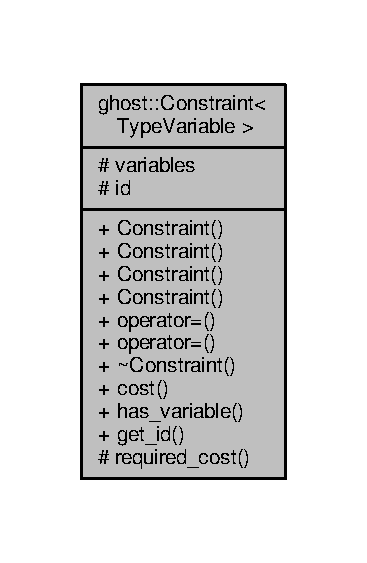
\includegraphics[width=226pt]{classghost_1_1Constraint__coll__graph}
\end{center}
\end{figure}
\subsection*{Public Member Functions}
\begin{DoxyCompactItemize}
\item 
\hyperlink{classghost_1_1Constraint_af2b5d5f541f64e548bc6c93bba1ba2b8}{Constraint} (const vector$<$ Type\-Variable $>$ $\ast$\hyperlink{classghost_1_1Constraint_a827e487bd77c8dbc4701d1dfae39678a}{variables}, const Type\-Domain $\ast$\hyperlink{classghost_1_1Constraint_a0ea15d113ab23ddb6ad74be72f7ac90d}{domain})
\begin{DoxyCompactList}\small\item\em The unique \hyperlink{classghost_1_1Constraint}{Constraint} constructor. \end{DoxyCompactList}\item 
double \hyperlink{classghost_1_1Constraint_a5051092934738b004fe848190a5aa9a5}{cost} (vector$<$ double $>$ \&var\-Cost) const 
\item 
vector$<$ double $>$ \hyperlink{classghost_1_1Constraint_a173958081ed2cfad938cead81b684455}{simulate\-Cost} (Type\-Variable \&current\-Var, const vector$<$ int $>$ \&possible\-Values, vector$<$ vector$<$ double $>$ $>$ \&vec\-Var\-Sim\-Costs, shared\-\_\-ptr$<$ \hyperlink{classghost_1_1Objective}{Objective}$<$ Type\-Variable, Type\-Domain $>$ $>$ objective)
\item 
vector$<$ double $>$ \hyperlink{classghost_1_1Constraint_ae5312daf02d5a4147dd4b519f2355712}{simulate\-Cost} (Type\-Variable \&current\-Var, const vector$<$ int $>$ \&possible\-Values, vector$<$ vector$<$ double $>$ $>$ \&vec\-Var\-Sim\-Costs)
\end{DoxyCompactItemize}
\subsection*{Protected Member Functions}
\begin{DoxyCompactItemize}
\item 
virtual double \hyperlink{classghost_1_1Constraint_ac67f7952cdf7212327b7db506225d12c}{v\-\_\-cost} (vector$<$ double $>$ \&var\-Cost) const =0
\begin{DoxyCompactList}\small\item\em Pure virtual function to compute the current cost of the constraint. \end{DoxyCompactList}\item 
virtual vector$<$ double $>$ \hyperlink{classghost_1_1Constraint_a8dd05c04dbce51e88a6301e9332fb2f5}{v\-\_\-simulate\-Cost} (Type\-Variable \&current\-Var, const vector$<$ int $>$ \&possible\-Values, vector$<$ vector$<$ double $>$ $>$ \&vec\-Var\-Sim\-Costs, shared\-\_\-ptr$<$ \hyperlink{classghost_1_1Objective}{Objective}$<$ Type\-Variable, Type\-Domain $>$ $>$ objective)=0
\begin{DoxyCompactList}\small\item\em Pure virtual function to simulate the cost of the constraint on all possible values of the given variable. \end{DoxyCompactList}\end{DoxyCompactItemize}
\subsection*{Protected Attributes}
\begin{DoxyCompactItemize}
\item 
vector$<$ Type\-Variable $>$ $\ast$ \hyperlink{classghost_1_1Constraint_a827e487bd77c8dbc4701d1dfae39678a}{variables}
\begin{DoxyCompactList}\small\item\em A pointer to the vector of variable objects of the C\-S\-P/\-C\-O\-P. \end{DoxyCompactList}\item 
Type\-Domain $\ast$ \hyperlink{classghost_1_1Constraint_a0ea15d113ab23ddb6ad74be72f7ac90d}{domain}
\begin{DoxyCompactList}\small\item\em A pointer to the domain object of the C\-S\-P/\-C\-O\-P. \end{DoxyCompactList}\end{DoxyCompactItemize}
\subsection*{Friends}
\begin{DoxyCompactItemize}
\item 
ostream \& \hyperlink{classghost_1_1Constraint_a5fb3db9a0881ff7aae65d680386277f0}{operator$<$$<$} (ostream \&os, const \hyperlink{classghost_1_1Constraint}{Constraint}$<$ Type\-Variable, Type\-Domain $>$ \&c)
\begin{DoxyCompactList}\small\item\em friend override of operator$<$$<$ \end{DoxyCompactList}\end{DoxyCompactItemize}


\subsection{Detailed Description}
\subsubsection*{template$<$typename Type\-Variable, typename Type\-Domain$>$class ghost\-::\-Constraint$<$ Type\-Variable, Type\-Domain $>$}

\hyperlink{classghost_1_1Constraint}{Constraint} is the class encoding constraints of your C\-S\-P/\-C\-O\-P. 

In G\-H\-O\-S\-T, many different constraint objects can be instanciate.

The \hyperlink{classghost_1_1Constraint}{Constraint} class is a template class, waiting for both the type of variable and the type of domain. Thus, you must instanciate a constraint by specifying the class of your variable objects and the class of your domain object, like for instance Constraint$<$\-Variable, Domain$>$ or \hyperlink{classghost_1_1Constraint}{Constraint}$<$My\-Custom\-Variable, My\-Custom\-Domain$>$, if My\-Custom\-Variable inherits from the \hyperlink{classghost_1_1Variable}{ghost\-::\-Variable} class and My\-Custom\-Domain inherits from the \hyperlink{classghost_1_1Domain}{ghost\-::\-Domain} class.

You cannot directly use this class \hyperlink{classghost_1_1Constraint}{Constraint} to encode your C\-S\-P/\-C\-O\-P constraints, since this is an abstract class (see the list of pure virtual functions below). Thus, you must write your own constraint class inheriting from \hyperlink{classghost_1_1Constraint}{ghost\-::\-Constraint}.

Pure virtual \hyperlink{classghost_1_1Constraint}{Constraint} functions\-:
\begin{DoxyItemize}
\item cost
\item simulate\-Cost
\end{DoxyItemize}

\begin{DoxySeeAlso}{See Also}
\hyperlink{classghost_1_1Variable}{Variable}, \hyperlink{classghost_1_1Domain}{Domain} 
\end{DoxySeeAlso}


\subsection{Constructor \& Destructor Documentation}
\hypertarget{classghost_1_1Constraint_af2b5d5f541f64e548bc6c93bba1ba2b8}{\index{ghost\-::\-Constraint@{ghost\-::\-Constraint}!Constraint@{Constraint}}
\index{Constraint@{Constraint}!ghost::Constraint@{ghost\-::\-Constraint}}
\subsubsection[{Constraint}]{\setlength{\rightskip}{0pt plus 5cm}template$<$typename Type\-Variable , typename Type\-Domain $>$ {\bf ghost\-::\-Constraint}$<$ Type\-Variable, Type\-Domain $>$\-::{\bf Constraint} (
\begin{DoxyParamCaption}
\item[{const vector$<$ Type\-Variable $>$ $\ast$}]{variables, }
\item[{const Type\-Domain $\ast$}]{domain}
\end{DoxyParamCaption}
)\hspace{0.3cm}{\ttfamily [inline]}}}\label{classghost_1_1Constraint_af2b5d5f541f64e548bc6c93bba1ba2b8}


The unique \hyperlink{classghost_1_1Constraint}{Constraint} constructor. 


\begin{DoxyParams}{Parameters}
{\em variables} & A constant pointer toward the vector of variable objects of the C\-S\-P/\-C\-O\-P. \\
\hline
{\em domain} & A constant pointer toward the domain object of the C\-S\-P/\-C\-O\-P. \\
\hline
\end{DoxyParams}


\subsection{Member Function Documentation}
\hypertarget{classghost_1_1Constraint_a5051092934738b004fe848190a5aa9a5}{\index{ghost\-::\-Constraint@{ghost\-::\-Constraint}!cost@{cost}}
\index{cost@{cost}!ghost::Constraint@{ghost\-::\-Constraint}}
\subsubsection[{cost}]{\setlength{\rightskip}{0pt plus 5cm}template$<$typename Type\-Variable , typename Type\-Domain $>$ double {\bf ghost\-::\-Constraint}$<$ Type\-Variable, Type\-Domain $>$\-::cost (
\begin{DoxyParamCaption}
\item[{vector$<$ double $>$ \&}]{var\-Cost}
\end{DoxyParamCaption}
) const\hspace{0.3cm}{\ttfamily [inline]}}}\label{classghost_1_1Constraint_a5051092934738b004fe848190a5aa9a5}
Inline function following the N\-V\-I idiom. Calling v\-\_\-cost. \begin{DoxySeeAlso}{See Also}
\hyperlink{classghost_1_1Constraint_ac67f7952cdf7212327b7db506225d12c}{v\-\_\-cost} 
\end{DoxySeeAlso}
\hypertarget{classghost_1_1Constraint_a173958081ed2cfad938cead81b684455}{\index{ghost\-::\-Constraint@{ghost\-::\-Constraint}!simulate\-Cost@{simulate\-Cost}}
\index{simulate\-Cost@{simulate\-Cost}!ghost::Constraint@{ghost\-::\-Constraint}}
\subsubsection[{simulate\-Cost}]{\setlength{\rightskip}{0pt plus 5cm}template$<$typename Type\-Variable , typename Type\-Domain $>$ vector$<$double$>$ {\bf ghost\-::\-Constraint}$<$ Type\-Variable, Type\-Domain $>$\-::simulate\-Cost (
\begin{DoxyParamCaption}
\item[{Type\-Variable \&}]{current\-Var, }
\item[{const vector$<$ int $>$ \&}]{possible\-Values, }
\item[{vector$<$ vector$<$ double $>$ $>$ \&}]{vec\-Var\-Sim\-Costs, }
\item[{shared\-\_\-ptr$<$ {\bf Objective}$<$ Type\-Variable, Type\-Domain $>$ $>$}]{objective}
\end{DoxyParamCaption}
)\hspace{0.3cm}{\ttfamily [inline]}}}\label{classghost_1_1Constraint_a173958081ed2cfad938cead81b684455}
Inline function following the N\-V\-I idiom. Calling v\-\_\-simulte\-Cost. \begin{DoxySeeAlso}{See Also}
v\-\_\-simulte\-Cost 
\end{DoxySeeAlso}
\hypertarget{classghost_1_1Constraint_ae5312daf02d5a4147dd4b519f2355712}{\index{ghost\-::\-Constraint@{ghost\-::\-Constraint}!simulate\-Cost@{simulate\-Cost}}
\index{simulate\-Cost@{simulate\-Cost}!ghost::Constraint@{ghost\-::\-Constraint}}
\subsubsection[{simulate\-Cost}]{\setlength{\rightskip}{0pt plus 5cm}template$<$typename Type\-Variable , typename Type\-Domain $>$ vector$<$double$>$ {\bf ghost\-::\-Constraint}$<$ Type\-Variable, Type\-Domain $>$\-::simulate\-Cost (
\begin{DoxyParamCaption}
\item[{Type\-Variable \&}]{current\-Var, }
\item[{const vector$<$ int $>$ \&}]{possible\-Values, }
\item[{vector$<$ vector$<$ double $>$ $>$ \&}]{vec\-Var\-Sim\-Costs}
\end{DoxyParamCaption}
)\hspace{0.3cm}{\ttfamily [inline]}}}\label{classghost_1_1Constraint_ae5312daf02d5a4147dd4b519f2355712}
Inline function following the N\-V\-I idiom, with objective = nullptr. Calling v\-\_\-simulte\-Cost. \begin{DoxySeeAlso}{See Also}
v\-\_\-simulte\-Cost 
\end{DoxySeeAlso}
\hypertarget{classghost_1_1Constraint_ac67f7952cdf7212327b7db506225d12c}{\index{ghost\-::\-Constraint@{ghost\-::\-Constraint}!v\-\_\-cost@{v\-\_\-cost}}
\index{v\-\_\-cost@{v\-\_\-cost}!ghost::Constraint@{ghost\-::\-Constraint}}
\subsubsection[{v\-\_\-cost}]{\setlength{\rightskip}{0pt plus 5cm}template$<$typename Type\-Variable , typename Type\-Domain $>$ virtual double {\bf ghost\-::\-Constraint}$<$ Type\-Variable, Type\-Domain $>$\-::v\-\_\-cost (
\begin{DoxyParamCaption}
\item[{vector$<$ double $>$ \&}]{var\-Cost}
\end{DoxyParamCaption}
) const\hspace{0.3cm}{\ttfamily [protected]}, {\ttfamily [pure virtual]}}}\label{classghost_1_1Constraint_ac67f7952cdf7212327b7db506225d12c}


Pure virtual function to compute the current cost of the constraint. 

In cost, the parameter var\-Cost is not given to be used by the function, but to store into var\-Cost the projected cost of each variable. This must be computed I\-N\-S\-I\-D\-E the cost function.


\begin{DoxyParams}{Parameters}
{\em var\-Cost} & A reference to a vector of double in order to store the projected cost of each variable. \\
\hline
\end{DoxyParams}
\begin{DoxyReturn}{Returns}
A double representing the cost of the constraint on the current configuration. 
\end{DoxyReturn}
\begin{DoxySeeAlso}{See Also}
\hyperlink{classghost_1_1Constraint_a5051092934738b004fe848190a5aa9a5}{cost} \hyperlink{classghost_1_1Constraint_a8dd05c04dbce51e88a6301e9332fb2f5}{v\-\_\-simulate\-Cost} 
\end{DoxySeeAlso}
\hypertarget{classghost_1_1Constraint_a8dd05c04dbce51e88a6301e9332fb2f5}{\index{ghost\-::\-Constraint@{ghost\-::\-Constraint}!v\-\_\-simulate\-Cost@{v\-\_\-simulate\-Cost}}
\index{v\-\_\-simulate\-Cost@{v\-\_\-simulate\-Cost}!ghost::Constraint@{ghost\-::\-Constraint}}
\subsubsection[{v\-\_\-simulate\-Cost}]{\setlength{\rightskip}{0pt plus 5cm}template$<$typename Type\-Variable , typename Type\-Domain $>$ virtual vector$<$double$>$ {\bf ghost\-::\-Constraint}$<$ Type\-Variable, Type\-Domain $>$\-::v\-\_\-simulate\-Cost (
\begin{DoxyParamCaption}
\item[{Type\-Variable \&}]{current\-Var, }
\item[{const vector$<$ int $>$ \&}]{possible\-Values, }
\item[{vector$<$ vector$<$ double $>$ $>$ \&}]{vec\-Var\-Sim\-Costs, }
\item[{shared\-\_\-ptr$<$ {\bf Objective}$<$ Type\-Variable, Type\-Domain $>$ $>$}]{objective}
\end{DoxyParamCaption}
)\hspace{0.3cm}{\ttfamily [protected]}, {\ttfamily [pure virtual]}}}\label{classghost_1_1Constraint_a8dd05c04dbce51e88a6301e9332fb2f5}


Pure virtual function to simulate the cost of the constraint on all possible values of the given variable. 

In v\-\_\-simulates\-Cost, the parameter vec\-Var\-Sim\-Costs is not given to be used by the function, but to store into vec\-Var\-Sim\-Costs the projected cost of current\-Var on all possible values. This must be computed I\-N\-S\-I\-D\-E the simulate\-Cost function.


\begin{DoxyParams}{Parameters}
{\em current\-Var} & A reference to the variable we want to change the current value. \\
\hline
{\em possible\-Values} & A reference to a constant vector of the possible values for current\-Var. \\
\hline
{\em vec\-Var\-Sim\-Costs} & A reference to the vector of vector of double in order to store the projected cost of current\-Var on all possible values. \\
\hline
{\em objective} & The (plausibly null) current objective object. This parameter is necessary to update the heuristic value helper. \\
\hline
\end{DoxyParams}
\begin{DoxyReturn}{Returns}
The vector of the cost of the constraint for each possible value of current\-Var. 
\end{DoxyReturn}
\begin{DoxySeeAlso}{See Also}
\hyperlink{classghost_1_1Constraint_a173958081ed2cfad938cead81b684455}{simulate\-Cost} \hyperlink{classghost_1_1Constraint_ac67f7952cdf7212327b7db506225d12c}{v\-\_\-cost} 
\end{DoxySeeAlso}


\subsection{Friends And Related Function Documentation}
\hypertarget{classghost_1_1Constraint_a5fb3db9a0881ff7aae65d680386277f0}{\index{ghost\-::\-Constraint@{ghost\-::\-Constraint}!operator$<$$<$@{operator$<$$<$}}
\index{operator$<$$<$@{operator$<$$<$}!ghost::Constraint@{ghost\-::\-Constraint}}
\subsubsection[{operator$<$$<$}]{\setlength{\rightskip}{0pt plus 5cm}template$<$typename Type\-Variable , typename Type\-Domain $>$ ostream\& operator$<$$<$ (
\begin{DoxyParamCaption}
\item[{ostream \&}]{os, }
\item[{const {\bf Constraint}$<$ Type\-Variable, Type\-Domain $>$ \&}]{c}
\end{DoxyParamCaption}
)\hspace{0.3cm}{\ttfamily [friend]}}}\label{classghost_1_1Constraint_a5fb3db9a0881ff7aae65d680386277f0}


friend override of operator$<$$<$ 



\subsection{Member Data Documentation}
\hypertarget{classghost_1_1Constraint_a0ea15d113ab23ddb6ad74be72f7ac90d}{\index{ghost\-::\-Constraint@{ghost\-::\-Constraint}!domain@{domain}}
\index{domain@{domain}!ghost::Constraint@{ghost\-::\-Constraint}}
\subsubsection[{domain}]{\setlength{\rightskip}{0pt plus 5cm}template$<$typename Type\-Variable , typename Type\-Domain $>$ Type\-Domain$\ast$ {\bf ghost\-::\-Constraint}$<$ Type\-Variable, Type\-Domain $>$\-::domain\hspace{0.3cm}{\ttfamily [protected]}}}\label{classghost_1_1Constraint_a0ea15d113ab23ddb6ad74be72f7ac90d}


A pointer to the domain object of the C\-S\-P/\-C\-O\-P. 

\hypertarget{classghost_1_1Constraint_a827e487bd77c8dbc4701d1dfae39678a}{\index{ghost\-::\-Constraint@{ghost\-::\-Constraint}!variables@{variables}}
\index{variables@{variables}!ghost::Constraint@{ghost\-::\-Constraint}}
\subsubsection[{variables}]{\setlength{\rightskip}{0pt plus 5cm}template$<$typename Type\-Variable , typename Type\-Domain $>$ vector$<$ Type\-Variable $>$$\ast$ {\bf ghost\-::\-Constraint}$<$ Type\-Variable, Type\-Domain $>$\-::variables\hspace{0.3cm}{\ttfamily [protected]}}}\label{classghost_1_1Constraint_a827e487bd77c8dbc4701d1dfae39678a}


A pointer to the vector of variable objects of the C\-S\-P/\-C\-O\-P. 



The documentation for this class was generated from the following file\-:\begin{DoxyCompactItemize}
\item 
include/constraints/\hyperlink{constraint_8hpp}{constraint.\-hpp}\end{DoxyCompactItemize}

\hypertarget{classghost_1_1Domain}{}\section{ghost\+:\+:Domain Class Reference}
\label{classghost_1_1Domain}\index{ghost\+::\+Domain@{ghost\+::\+Domain}}


\hyperlink{classghost_1_1Domain}{Domain} is the class encoding the domain of your C\+S\+P/\+C\+OP.  




{\ttfamily \#include $<$domain.\+hpp$>$}



Collaboration diagram for ghost\+:\+:Domain\+:\nopagebreak
\begin{figure}[H]
\begin{center}
\leavevmode
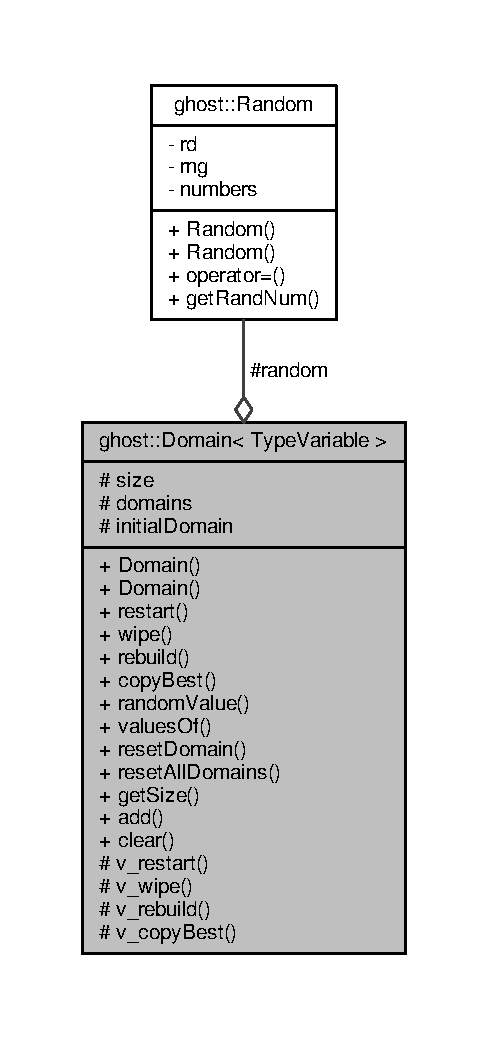
\includegraphics[width=172pt]{classghost_1_1Domain__coll__graph}
\end{center}
\end{figure}
\subsection*{Public Member Functions}
\begin{DoxyCompactItemize}
\item 
\hyperlink{classghost_1_1Domain_adbdf32b7d0129175ec320f4b7c10132e}{Domain} (const vector$<$ int $>$ \&domain)
\begin{DoxyCompactList}\small\item\em First \hyperlink{classghost_1_1Domain}{Domain} constructor. \end{DoxyCompactList}\item 
\hyperlink{classghost_1_1Domain_a6a9f7b0aec78acb0b0f4edefaea7a6e9}{Domain} (int size, int start\+Value)
\begin{DoxyCompactList}\small\item\em Second \hyperlink{classghost_1_1Domain}{Domain} constructor. \end{DoxyCompactList}\item 
\hyperlink{classghost_1_1Domain_ae2419e072b48d1aaa5e9aedc36babbb6}{Domain} (const \hyperlink{classghost_1_1Domain}{Domain} \&other)
\begin{DoxyCompactList}\small\item\em \hyperlink{classghost_1_1Domain}{Domain} copy constructor. \end{DoxyCompactList}\item 
\hyperlink{classghost_1_1Domain}{Domain} \& \hyperlink{classghost_1_1Domain_a69c6fb58d1811b8306d1dc8b0aaa6778}{operator=} (\hyperlink{classghost_1_1Domain}{Domain} other)
\begin{DoxyCompactList}\small\item\em \hyperlink{classghost_1_1Domain}{Domain}\textquotesingle{}s copy assignment operator. \end{DoxyCompactList}\item 
\hyperlink{classghost_1_1Domain_aa5d4791c2f90c021d9f19746f4694039}{$\sim$\+Domain} ()=default
\begin{DoxyCompactList}\small\item\em \hyperlink{classghost_1_1Domain}{Domain} destructor. \end{DoxyCompactList}\item 
int \hyperlink{classghost_1_1Domain_a5d12f840be7a0ddd673c85d70426a75e}{random\+\_\+value} () const 
\begin{DoxyCompactList}\small\item\em Inline function returning a random value from the domain, following a uniform distribution. \end{DoxyCompactList}\item 
size\+\_\+t \hyperlink{classghost_1_1Domain_a222990a926a5313aef33025d48b41712}{get\+\_\+size} () const 
\begin{DoxyCompactList}\small\item\em Inline function to get the size of the domain. \end{DoxyCompactList}\item 
const vector$<$ int $>$ \& \hyperlink{classghost_1_1Domain_af14587da3669db692a9b988cc240999a}{get\+\_\+domain} () const 
\begin{DoxyCompactList}\small\item\em Inline function to get the full domain. \end{DoxyCompactList}\item 
int \hyperlink{classghost_1_1Domain_a6e50fc11a5ed2857fccb69f12c0fa07d}{get\+\_\+value} (int index) const 
\begin{DoxyCompactList}\small\item\em Get the value at the given index. \end{DoxyCompactList}\item 
int \hyperlink{classghost_1_1Domain_a1201d3b7c15381d19510a131d8823ff0}{index\+\_\+of} (int value) const 
\begin{DoxyCompactList}\small\item\em Get the index of a given value. \end{DoxyCompactList}\end{DoxyCompactItemize}
\subsection*{Friends}
\begin{DoxyCompactItemize}
\item 
ostream \& \hyperlink{classghost_1_1Domain_a608c9910828eb2983efb65ff4c297a4e}{operator$<$$<$} (ostream \&os, const \hyperlink{classghost_1_1Domain}{Domain} \&domain)
\end{DoxyCompactItemize}


\subsection{Detailed Description}
\hyperlink{classghost_1_1Domain}{Domain} is the class encoding the domain of your C\+S\+P/\+C\+OP. 

\hyperlink{classghost_1_1Domain}{Domain} is the class implementing variable domains, ie, the set of possible values a variable can take. In G\+H\+O\+ST, such values must be integers. 

\subsection{Constructor \& Destructor Documentation}
\index{ghost\+::\+Domain@{ghost\+::\+Domain}!Domain@{Domain}}
\index{Domain@{Domain}!ghost\+::\+Domain@{ghost\+::\+Domain}}
\subsubsection[{\texorpdfstring{Domain(const vector$<$ int $>$ \&domain)}{Domain(const vector< int > &domain)}}]{\setlength{\rightskip}{0pt plus 5cm}ghost\+::\+Domain\+::\+Domain (
\begin{DoxyParamCaption}
\item[{const vector$<$ int $>$ \&}]{domain}
\end{DoxyParamCaption}
)}\hypertarget{classghost_1_1Domain_adbdf32b7d0129175ec320f4b7c10132e}{}\label{classghost_1_1Domain_adbdf32b7d0129175ec320f4b7c10132e}


First \hyperlink{classghost_1_1Domain}{Domain} constructor. 

Constructor taking a vector of integer values.


\begin{DoxyParams}{Parameters}
{\em domain} & A vector of int corresponding to the variable domain. \\
\hline
\end{DoxyParams}
\index{ghost\+::\+Domain@{ghost\+::\+Domain}!Domain@{Domain}}
\index{Domain@{Domain}!ghost\+::\+Domain@{ghost\+::\+Domain}}
\subsubsection[{\texorpdfstring{Domain(int size, int start\+Value)}{Domain(int size, int startValue)}}]{\setlength{\rightskip}{0pt plus 5cm}ghost\+::\+Domain\+::\+Domain (
\begin{DoxyParamCaption}
\item[{int}]{size, }
\item[{int}]{start\+Value}
\end{DoxyParamCaption}
)}\hypertarget{classghost_1_1Domain_a6a9f7b0aec78acb0b0f4edefaea7a6e9}{}\label{classghost_1_1Domain_a6a9f7b0aec78acb0b0f4edefaea7a6e9}


Second \hyperlink{classghost_1_1Domain}{Domain} constructor. 

Constructor taking the domain of size \textquotesingle{}size\textquotesingle{} and a starting value \textquotesingle{}star\+Value\textquotesingle{}, thus creating a domain with all integer values in \mbox{[}x, x + N\mbox{]}.


\begin{DoxyParams}{Parameters}
{\em size} & An integer specifying the size of the domain. \\
\hline
{\em start\+Value} & An integer specifying what is the first value in the domain. \\
\hline
\end{DoxyParams}
\index{ghost\+::\+Domain@{ghost\+::\+Domain}!Domain@{Domain}}
\index{Domain@{Domain}!ghost\+::\+Domain@{ghost\+::\+Domain}}
\subsubsection[{\texorpdfstring{Domain(const Domain \&other)}{Domain(const Domain &other)}}]{\setlength{\rightskip}{0pt plus 5cm}ghost\+::\+Domain\+::\+Domain (
\begin{DoxyParamCaption}
\item[{const {\bf Domain} \&}]{other}
\end{DoxyParamCaption}
)}\hypertarget{classghost_1_1Domain_ae2419e072b48d1aaa5e9aedc36babbb6}{}\label{classghost_1_1Domain_ae2419e072b48d1aaa5e9aedc36babbb6}


\hyperlink{classghost_1_1Domain}{Domain} copy constructor. 


\begin{DoxyParams}{Parameters}
{\em other} & A const reference to a \hyperlink{classghost_1_1Domain}{Domain} object. \\
\hline
\end{DoxyParams}
\index{ghost\+::\+Domain@{ghost\+::\+Domain}!````~Domain@{$\sim$\+Domain}}
\index{````~Domain@{$\sim$\+Domain}!ghost\+::\+Domain@{ghost\+::\+Domain}}
\subsubsection[{\texorpdfstring{$\sim$\+Domain()=default}{~Domain()=default}}]{\setlength{\rightskip}{0pt plus 5cm}ghost\+::\+Domain\+::$\sim$\+Domain (
\begin{DoxyParamCaption}
{}
\end{DoxyParamCaption}
)\hspace{0.3cm}{\ttfamily [default]}}\hypertarget{classghost_1_1Domain_aa5d4791c2f90c021d9f19746f4694039}{}\label{classghost_1_1Domain_aa5d4791c2f90c021d9f19746f4694039}


\hyperlink{classghost_1_1Domain}{Domain} destructor. 



\subsection{Member Function Documentation}
\index{ghost\+::\+Domain@{ghost\+::\+Domain}!get\+\_\+domain@{get\+\_\+domain}}
\index{get\+\_\+domain@{get\+\_\+domain}!ghost\+::\+Domain@{ghost\+::\+Domain}}
\subsubsection[{\texorpdfstring{get\+\_\+domain() const }{get_domain() const }}]{\setlength{\rightskip}{0pt plus 5cm}const vector$<$int$>$\& ghost\+::\+Domain\+::get\+\_\+domain (
\begin{DoxyParamCaption}
{}
\end{DoxyParamCaption}
) const\hspace{0.3cm}{\ttfamily [inline]}}\hypertarget{classghost_1_1Domain_af14587da3669db692a9b988cc240999a}{}\label{classghost_1_1Domain_af14587da3669db692a9b988cc240999a}


Inline function to get the full domain. 

\index{ghost\+::\+Domain@{ghost\+::\+Domain}!get\+\_\+size@{get\+\_\+size}}
\index{get\+\_\+size@{get\+\_\+size}!ghost\+::\+Domain@{ghost\+::\+Domain}}
\subsubsection[{\texorpdfstring{get\+\_\+size() const }{get_size() const }}]{\setlength{\rightskip}{0pt plus 5cm}size\+\_\+t ghost\+::\+Domain\+::get\+\_\+size (
\begin{DoxyParamCaption}
{}
\end{DoxyParamCaption}
) const\hspace{0.3cm}{\ttfamily [inline]}}\hypertarget{classghost_1_1Domain_a222990a926a5313aef33025d48b41712}{}\label{classghost_1_1Domain_a222990a926a5313aef33025d48b41712}


Inline function to get the size of the domain. 

Get the number of values currently composing the domain. \begin{DoxyReturn}{Returns}
A size\+\_\+t corresponding to the size of the domain. 
\end{DoxyReturn}
\index{ghost\+::\+Domain@{ghost\+::\+Domain}!get\+\_\+value@{get\+\_\+value}}
\index{get\+\_\+value@{get\+\_\+value}!ghost\+::\+Domain@{ghost\+::\+Domain}}
\subsubsection[{\texorpdfstring{get\+\_\+value(int index) const }{get_value(int index) const }}]{\setlength{\rightskip}{0pt plus 5cm}int ghost\+::\+Domain\+::get\+\_\+value (
\begin{DoxyParamCaption}
\item[{int}]{index}
\end{DoxyParamCaption}
) const}\hypertarget{classghost_1_1Domain_a6e50fc11a5ed2857fccb69f12c0fa07d}{}\label{classghost_1_1Domain_a6e50fc11a5ed2857fccb69f12c0fa07d}


Get the value at the given index. 


\begin{DoxyParams}{Parameters}
{\em index} & is the index of the desired value. \\
\hline
\end{DoxyParams}
\begin{DoxyReturn}{Returns}
The value at the given index if this one is in the range of the domain, raises an \hyperlink{structghost_1_1indexException}{index\+Exception} otherwise. 
\end{DoxyReturn}
\index{ghost\+::\+Domain@{ghost\+::\+Domain}!index\+\_\+of@{index\+\_\+of}}
\index{index\+\_\+of@{index\+\_\+of}!ghost\+::\+Domain@{ghost\+::\+Domain}}
\subsubsection[{\texorpdfstring{index\+\_\+of(int value) const }{index_of(int value) const }}]{\setlength{\rightskip}{0pt plus 5cm}int ghost\+::\+Domain\+::index\+\_\+of (
\begin{DoxyParamCaption}
\item[{int}]{value}
\end{DoxyParamCaption}
) const}\hypertarget{classghost_1_1Domain_a1201d3b7c15381d19510a131d8823ff0}{}\label{classghost_1_1Domain_a1201d3b7c15381d19510a131d8823ff0}


Get the index of a given value. 

\begin{DoxyReturn}{Returns}
Returns its index if the given value is in the domain, or raises a \hyperlink{structghost_1_1valueException}{value\+Exception} otherwise. 
\end{DoxyReturn}
\index{ghost\+::\+Domain@{ghost\+::\+Domain}!operator=@{operator=}}
\index{operator=@{operator=}!ghost\+::\+Domain@{ghost\+::\+Domain}}
\subsubsection[{\texorpdfstring{operator=(\+Domain other)}{operator=(Domain other)}}]{\setlength{\rightskip}{0pt plus 5cm}{\bf Domain}\& ghost\+::\+Domain\+::operator= (
\begin{DoxyParamCaption}
\item[{{\bf Domain}}]{other}
\end{DoxyParamCaption}
)}\hypertarget{classghost_1_1Domain_a69c6fb58d1811b8306d1dc8b0aaa6778}{}\label{classghost_1_1Domain_a69c6fb58d1811b8306d1dc8b0aaa6778}


\hyperlink{classghost_1_1Domain}{Domain}\textquotesingle{}s copy assignment operator. 

The copy-\/and-\/swap idiom is applyed here.


\begin{DoxyParams}{Parameters}
{\em other} & A \hyperlink{classghost_1_1Domain}{Domain} object. \\
\hline
\end{DoxyParams}
\index{ghost\+::\+Domain@{ghost\+::\+Domain}!random\+\_\+value@{random\+\_\+value}}
\index{random\+\_\+value@{random\+\_\+value}!ghost\+::\+Domain@{ghost\+::\+Domain}}
\subsubsection[{\texorpdfstring{random\+\_\+value() const }{random_value() const }}]{\setlength{\rightskip}{0pt plus 5cm}int ghost\+::\+Domain\+::random\+\_\+value (
\begin{DoxyParamCaption}
{}
\end{DoxyParamCaption}
) const\hspace{0.3cm}{\ttfamily [inline]}}\hypertarget{classghost_1_1Domain_a5d12f840be7a0ddd673c85d70426a75e}{}\label{classghost_1_1Domain_a5d12f840be7a0ddd673c85d70426a75e}


Inline function returning a random value from the domain, following a uniform distribution. 



\subsection{Friends And Related Function Documentation}
\index{ghost\+::\+Domain@{ghost\+::\+Domain}!operator$<$$<$@{operator$<$$<$}}
\index{operator$<$$<$@{operator$<$$<$}!ghost\+::\+Domain@{ghost\+::\+Domain}}
\subsubsection[{\texorpdfstring{operator$<$$<$}{operator<<}}]{\setlength{\rightskip}{0pt plus 5cm}ostream\& operator$<$$<$ (
\begin{DoxyParamCaption}
\item[{ostream \&}]{os, }
\item[{const {\bf Domain} \&}]{domain}
\end{DoxyParamCaption}
)\hspace{0.3cm}{\ttfamily [friend]}}\hypertarget{classghost_1_1Domain_a608c9910828eb2983efb65ff4c297a4e}{}\label{classghost_1_1Domain_a608c9910828eb2983efb65ff4c297a4e}


The documentation for this class was generated from the following file\+:\begin{DoxyCompactItemize}
\item 
include/\hyperlink{domain_8hpp}{domain.\+hpp}\end{DoxyCompactItemize}

\hypertarget{classghost_1_1NullObjective}{\section{ghost\-:\-:Null\-Objective$<$ Type\-Variable, Type\-Domain $>$ Class Template Reference}
\label{classghost_1_1NullObjective}\index{ghost\-::\-Null\-Objective$<$ Type\-Variable, Type\-Domain $>$@{ghost\-::\-Null\-Objective$<$ Type\-Variable, Type\-Domain $>$}}
}


\hyperlink{classghost_1_1NullObjective}{Null\-Objective} is used when no objective functions have been given to the solver (ie, for pure satisfaction runs).  




{\ttfamily \#include $<$objective.\-hpp$>$}



Inheritance diagram for ghost\-:\-:Null\-Objective$<$ Type\-Variable, Type\-Domain $>$\-:\nopagebreak
\begin{figure}[H]
\begin{center}
\leavevmode
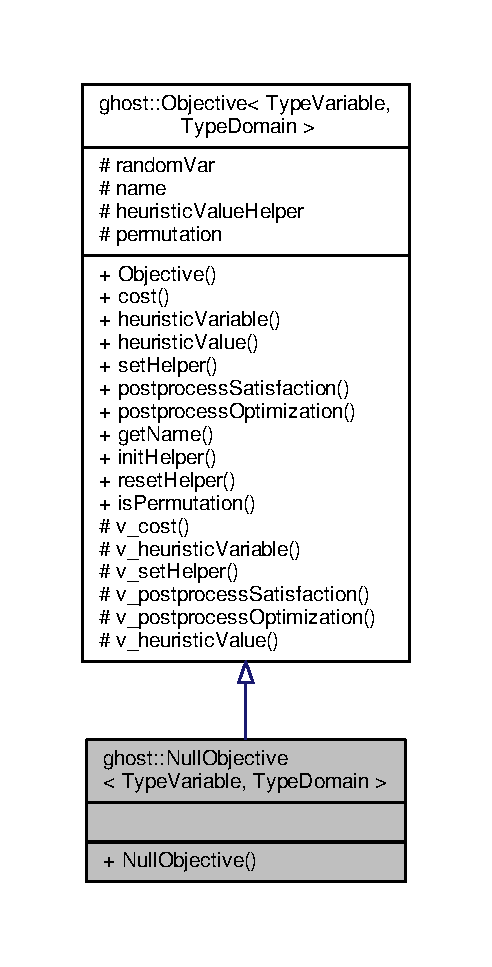
\includegraphics[width=236pt]{classghost_1_1NullObjective__inherit__graph}
\end{center}
\end{figure}


Collaboration diagram for ghost\-:\-:Null\-Objective$<$ Type\-Variable, Type\-Domain $>$\-:\nopagebreak
\begin{figure}[H]
\begin{center}
\leavevmode
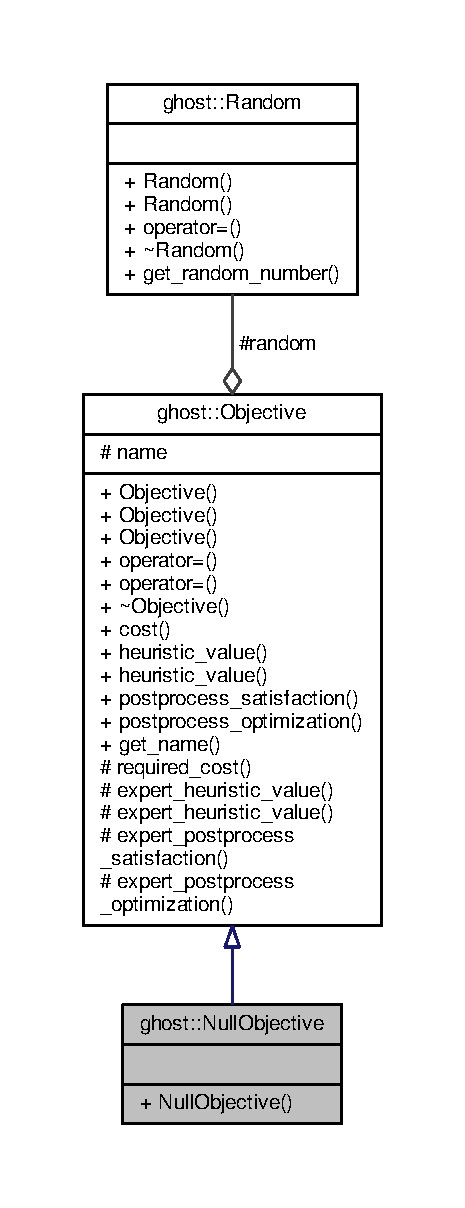
\includegraphics[height=550pt]{classghost_1_1NullObjective__coll__graph}
\end{center}
\end{figure}
\subsection*{Public Member Functions}
\begin{DoxyCompactItemize}
\item 
\hyperlink{classghost_1_1NullObjective_acb468a9e5fd85d31c3afc805481919ed}{Null\-Objective} ()
\end{DoxyCompactItemize}
\subsection*{Private Member Functions}
\begin{DoxyCompactItemize}
\item 
virtual double \hyperlink{classghost_1_1NullObjective_a309e1913d38d728b41a61c1ce40f3dca}{v\-\_\-cost} (const vector$<$ Type\-Variable $>$ $\ast$vec\-Variables, const Type\-Domain $\ast$domain) const 
\begin{DoxyCompactList}\small\item\em Pure virtual function to compute the value of the objective function on the current configuration. \end{DoxyCompactList}\item 
virtual int \hyperlink{classghost_1_1NullObjective_aef7e24c71f2522034764402704e3b16f}{v\-\_\-heuristic\-Variable} (const vector$<$ int $>$ \&vec\-Id, const vector$<$ Type\-Variable $>$ $\ast$vec\-Variables, Type\-Domain $\ast$domain)
\begin{DoxyCompactList}\small\item\em Pure virtual function to apply the variable heuristic used by the solver. \end{DoxyCompactList}\item 
virtual void \hyperlink{classghost_1_1NullObjective_a5f4b22306c25132590e3c10a6dc34d15}{v\-\_\-set\-Helper} (const Type\-Variable \&b, const vector$<$ Type\-Variable $>$ $\ast$vec\-Variables, const Type\-Domain $\ast$domain)
\begin{DoxyCompactList}\small\item\em Pure virtual function to set heuristic\-Value\-Helper\mbox{[}current\-Var.\-get\-Value()\mbox{]}. \end{DoxyCompactList}\end{DoxyCompactItemize}
\subsection*{Additional Inherited Members}


\subsection{Detailed Description}
\subsubsection*{template$<$typename Type\-Variable, typename Type\-Domain$>$class ghost\-::\-Null\-Objective$<$ Type\-Variable, Type\-Domain $>$}

\hyperlink{classghost_1_1NullObjective}{Null\-Objective} is used when no objective functions have been given to the solver (ie, for pure satisfaction runs). 

\subsection{Constructor \& Destructor Documentation}
\hypertarget{classghost_1_1NullObjective_acb468a9e5fd85d31c3afc805481919ed}{\index{ghost\-::\-Null\-Objective@{ghost\-::\-Null\-Objective}!Null\-Objective@{Null\-Objective}}
\index{Null\-Objective@{Null\-Objective}!ghost::NullObjective@{ghost\-::\-Null\-Objective}}
\subsubsection[{Null\-Objective}]{\setlength{\rightskip}{0pt plus 5cm}template$<$typename Type\-Variable , typename Type\-Domain $>$ {\bf ghost\-::\-Null\-Objective}$<$ Type\-Variable, Type\-Domain $>$\-::{\bf Null\-Objective} (
\begin{DoxyParamCaption}
{}
\end{DoxyParamCaption}
)\hspace{0.3cm}{\ttfamily [inline]}}}\label{classghost_1_1NullObjective_acb468a9e5fd85d31c3afc805481919ed}


\subsection{Member Function Documentation}
\hypertarget{classghost_1_1NullObjective_a309e1913d38d728b41a61c1ce40f3dca}{\index{ghost\-::\-Null\-Objective@{ghost\-::\-Null\-Objective}!v\-\_\-cost@{v\-\_\-cost}}
\index{v\-\_\-cost@{v\-\_\-cost}!ghost::NullObjective@{ghost\-::\-Null\-Objective}}
\subsubsection[{v\-\_\-cost}]{\setlength{\rightskip}{0pt plus 5cm}template$<$typename Type\-Variable , typename Type\-Domain $>$ virtual double {\bf ghost\-::\-Null\-Objective}$<$ Type\-Variable, Type\-Domain $>$\-::v\-\_\-cost (
\begin{DoxyParamCaption}
\item[{const vector$<$ Type\-Variable $>$ $\ast$}]{vec\-Variables, }
\item[{const Type\-Domain $\ast$}]{domain}
\end{DoxyParamCaption}
) const\hspace{0.3cm}{\ttfamily [inline]}, {\ttfamily [private]}, {\ttfamily [virtual]}}}\label{classghost_1_1NullObjective_a309e1913d38d728b41a61c1ce40f3dca}


Pure virtual function to compute the value of the objective function on the current configuration. 


\begin{DoxyParams}{Parameters}
{\em vec\-Variables} & A constant pointer to the vector of variable objects of the C\-S\-P/\-C\-O\-P. \\
\hline
{\em domain} & A constant pointer to the domain object of the C\-S\-P/\-C\-O\-P. \\
\hline
\end{DoxyParams}
\begin{DoxyReturn}{Returns}
The value of the objective function on the current configuration. 
\end{DoxyReturn}
\begin{DoxySeeAlso}{See Also}
\hyperlink{classghost_1_1Objective_a2947c19e26ffd2a23c3a7f1b99c8bc79}{cost} 
\end{DoxySeeAlso}


Implements \hyperlink{classghost_1_1Objective_affb6d6730adfbfe6a1f990e00d2a5eb2}{ghost\-::\-Objective$<$ Type\-Variable, Type\-Domain $>$}.

\hypertarget{classghost_1_1NullObjective_aef7e24c71f2522034764402704e3b16f}{\index{ghost\-::\-Null\-Objective@{ghost\-::\-Null\-Objective}!v\-\_\-heuristic\-Variable@{v\-\_\-heuristic\-Variable}}
\index{v\-\_\-heuristic\-Variable@{v\-\_\-heuristic\-Variable}!ghost::NullObjective@{ghost\-::\-Null\-Objective}}
\subsubsection[{v\-\_\-heuristic\-Variable}]{\setlength{\rightskip}{0pt plus 5cm}template$<$typename Type\-Variable , typename Type\-Domain $>$ virtual int {\bf ghost\-::\-Null\-Objective}$<$ Type\-Variable, Type\-Domain $>$\-::v\-\_\-heuristic\-Variable (
\begin{DoxyParamCaption}
\item[{const vector$<$ int $>$ \&}]{vec\-Var\-Id, }
\item[{const vector$<$ Type\-Variable $>$ $\ast$}]{vec\-Variables, }
\item[{Type\-Domain $\ast$}]{domain}
\end{DoxyParamCaption}
)\hspace{0.3cm}{\ttfamily [inline]}, {\ttfamily [private]}, {\ttfamily [virtual]}}}\label{classghost_1_1NullObjective_aef7e24c71f2522034764402704e3b16f}


Pure virtual function to apply the variable heuristic used by the solver. 


\begin{DoxyParams}{Parameters}
{\em vec\-Var\-Id} & A constant reference to the vector of variable I\-D objects of the C\-S\-P/\-C\-O\-P. \\
\hline
{\em vec\-Variables} & A constant pointer to the vector of variable objects of the C\-S\-P/\-C\-O\-P. \\
\hline
{\em domain} & A constant pointer to the domain object of the C\-S\-P/\-C\-O\-P. \\
\hline
\end{DoxyParams}
\begin{DoxyReturn}{Returns}
The I\-D of the selected variable according to the heuristic. 
\end{DoxyReturn}
\begin{DoxySeeAlso}{See Also}
\hyperlink{classghost_1_1Objective_af68c07a226162ea7f9ee01a0b00d3ae4}{heuristic\-Variable} 
\end{DoxySeeAlso}


Implements \hyperlink{classghost_1_1Objective_ae4a49d23569c367182f934c25a6c6103}{ghost\-::\-Objective$<$ Type\-Variable, Type\-Domain $>$}.

\hypertarget{classghost_1_1NullObjective_a5f4b22306c25132590e3c10a6dc34d15}{\index{ghost\-::\-Null\-Objective@{ghost\-::\-Null\-Objective}!v\-\_\-set\-Helper@{v\-\_\-set\-Helper}}
\index{v\-\_\-set\-Helper@{v\-\_\-set\-Helper}!ghost::NullObjective@{ghost\-::\-Null\-Objective}}
\subsubsection[{v\-\_\-set\-Helper}]{\setlength{\rightskip}{0pt plus 5cm}template$<$typename Type\-Variable , typename Type\-Domain $>$ virtual void {\bf ghost\-::\-Null\-Objective}$<$ Type\-Variable, Type\-Domain $>$\-::v\-\_\-set\-Helper (
\begin{DoxyParamCaption}
\item[{const Type\-Variable \&}]{current\-Var, }
\item[{const vector$<$ Type\-Variable $>$ $\ast$}]{vec\-Variables, }
\item[{const Type\-Domain $\ast$}]{domain}
\end{DoxyParamCaption}
)\hspace{0.3cm}{\ttfamily [inline]}, {\ttfamily [private]}, {\ttfamily [virtual]}}}\label{classghost_1_1NullObjective_a5f4b22306c25132590e3c10a6dc34d15}


Pure virtual function to set heuristic\-Value\-Helper\mbox{[}current\-Var.\-get\-Value()\mbox{]}. 


\begin{DoxyParams}{Parameters}
{\em current\-Var} & A constant reference to a variable object. \\
\hline
{\em vec\-Variables} & A constant pointer to the vector of variable objects of the C\-S\-P/\-C\-O\-P. \\
\hline
{\em domain} & A constant pointer to the domain object of the C\-S\-P/\-C\-O\-P. \\
\hline
\end{DoxyParams}
\begin{DoxySeeAlso}{See Also}
\hyperlink{classghost_1_1Objective_ab589c264cf391bab9005562f66a39797}{set\-Helper}, \hyperlink{classghost_1_1Objective_a9bfe64f13de15bba7f2fa3a662c02e27}{heuristic\-Value\-Helper} 
\end{DoxySeeAlso}


Implements \hyperlink{classghost_1_1Objective_a8c4efc1602123b28626a37c53e100a6e}{ghost\-::\-Objective$<$ Type\-Variable, Type\-Domain $>$}.



The documentation for this class was generated from the following file\-:\begin{DoxyCompactItemize}
\item 
include/objectives/\hyperlink{objective_8hpp}{objective.\-hpp}\end{DoxyCompactItemize}

\hypertarget{classghost_1_1Objective}{}\section{ghost\+:\+:Objective$<$ Type\+Variable $>$ Class Template Reference}
\label{classghost_1_1Objective}\index{ghost\+::\+Objective$<$ Type\+Variable $>$@{ghost\+::\+Objective$<$ Type\+Variable $>$}}


\hyperlink{classghost_1_1Objective}{Objective} is the class encoding objective functions of your C\+S\+P/\+C\+OP.  




{\ttfamily \#include $<$objective.\+hpp$>$}



Inheritance diagram for ghost\+:\+:Objective$<$ Type\+Variable $>$\+:\nopagebreak
\begin{figure}[H]
\begin{center}
\leavevmode
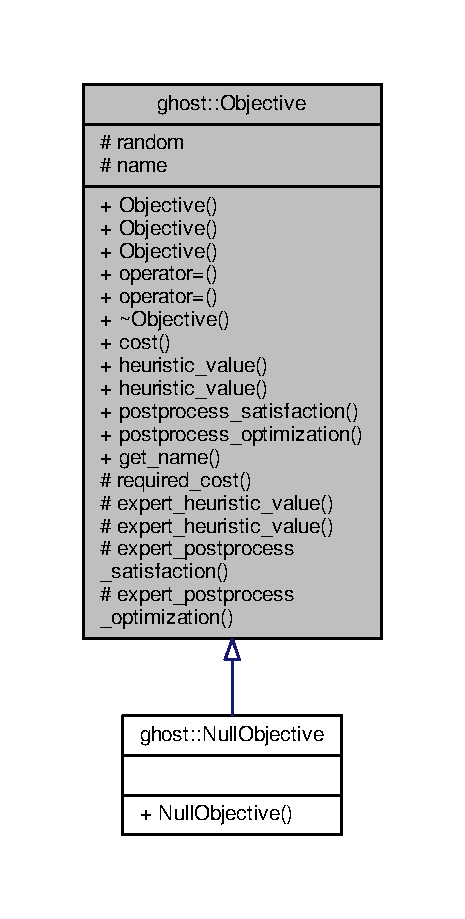
\includegraphics[width=243pt]{classghost_1_1Objective__inherit__graph}
\end{center}
\end{figure}


Collaboration diagram for ghost\+:\+:Objective$<$ Type\+Variable $>$\+:\nopagebreak
\begin{figure}[H]
\begin{center}
\leavevmode
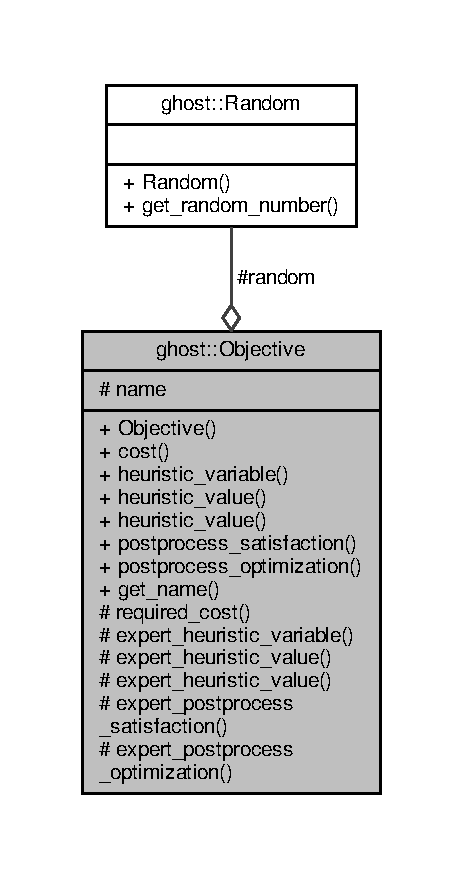
\includegraphics[width=243pt]{classghost_1_1Objective__coll__graph}
\end{center}
\end{figure}
\subsection*{Public Member Functions}
\begin{DoxyCompactItemize}
\item 
\hyperlink{classghost_1_1Objective_a05c72fc98983001626a5ffd4609fc4d1}{Objective} (const string \&\hyperlink{classghost_1_1Objective_a02aee324f6958b6c533f27ec430690fe}{name})
\begin{DoxyCompactList}\small\item\em The unique \hyperlink{classghost_1_1Objective}{Objective} constructor. \end{DoxyCompactList}\item 
\hyperlink{classghost_1_1Objective_a55b4f0ff2fdfc2ace35db536cc95ba20}{Objective} (const \hyperlink{classghost_1_1Objective}{Objective} \&other)=default
\begin{DoxyCompactList}\small\item\em Default copy and move contructors are explicitely declared. \end{DoxyCompactList}\item 
\hyperlink{classghost_1_1Objective_afb34a86055233acc3ebfb783f96a8e89}{Objective} (\hyperlink{classghost_1_1Objective}{Objective} \&\&other)=default
\item 
\hyperlink{classghost_1_1Objective}{Objective} \& \hyperlink{classghost_1_1Objective_a20f373a941afba7e3b6dbeb04ee4122d}{operator=} (const \hyperlink{classghost_1_1Objective}{Objective} \&other)=delete
\begin{DoxyCompactList}\small\item\em Copy and move assignment operators are disabled. \end{DoxyCompactList}\item 
\hyperlink{classghost_1_1Objective}{Objective} \& \hyperlink{classghost_1_1Objective_a8efc3f91216e6f50685e09da8cc3f04c}{operator=} (\hyperlink{classghost_1_1Objective}{Objective} \&\&other)=delete
\item 
virtual \hyperlink{classghost_1_1Objective_aade47b263cbe7cae55e237b423dc4895}{$\sim$\+Objective} ()=default
\item 
double \hyperlink{classghost_1_1Objective_ac46e9305c3a92db9dff2d233a7c07088}{cost} (vector$<$ Type\+Variable $>$ $\ast$variables) const 
\begin{DoxyCompactList}\small\item\em Inline function following the N\+VI idiom. Calling v\+\_\+cost. \end{DoxyCompactList}\item 
int \hyperlink{classghost_1_1Objective_ab9ed9b882b8e865d20eeae168001561a}{heuristic\+\_\+value} (vector$<$ Type\+Variable $>$ $\ast$variables, Type\+Variable $\ast$var, const vector$<$ int $>$ \&possible\+\_\+values) const 
\begin{DoxyCompactList}\small\item\em Inline function following the N\+VI idiom. Calling expert\+\_\+heuristic\+\_\+value. \end{DoxyCompactList}\item 
Type\+Variable $\ast$ \hyperlink{classghost_1_1Objective_ab52e4a66ce78c9477ef44b2d8dde57e6}{heuristic\+\_\+value} (vector$<$ Type\+Variable $\ast$ $>$ bad\+\_\+variables) const 
\begin{DoxyCompactList}\small\item\em Inline function following the N\+VI idiom. Calling expert\+\_\+heuristic\+\_\+value. \end{DoxyCompactList}\item 
void \hyperlink{classghost_1_1Objective_a953abf257ee236e934011754edada4a9}{postprocess\+\_\+satisfaction} (vector$<$ Type\+Variable $>$ $\ast$variables, double \&best\+Cost, vector$<$ int $>$ \&solution) const 
\begin{DoxyCompactList}\small\item\em Inline function following the N\+VI idiom. Calling expert\+\_\+postprocess\+\_\+satisfaction. \end{DoxyCompactList}\item 
void \hyperlink{classghost_1_1Objective_ae9e095cabcd99b2b0a7b1861ecf4ca20}{postprocess\+\_\+optimization} (vector$<$ Type\+Variable $>$ $\ast$variables, double \&best\+Cost, vector$<$ int $>$ \&solution) const 
\begin{DoxyCompactList}\small\item\em Inline function following the N\+VI idiom. Calling expert\+\_\+postprocess\+\_\+optimization. \end{DoxyCompactList}\item 
string \hyperlink{classghost_1_1Objective_aeb2af94526fac09e2c4242817b22ef09}{get\+\_\+name} () const 
\begin{DoxyCompactList}\small\item\em Inline accessor to get the name of the objective object. \end{DoxyCompactList}\end{DoxyCompactItemize}
\subsection*{Protected Member Functions}
\begin{DoxyCompactItemize}
\item 
virtual double \hyperlink{classghost_1_1Objective_ac6baed2eee899efd4c485e5a1e563ee9}{required\+\_\+cost} (vector$<$ Type\+Variable $>$ $\ast$variables) const =0
\begin{DoxyCompactList}\small\item\em Pure virtual function to compute the value of the objective function on the current configuration. \end{DoxyCompactList}\item 
virtual int \hyperlink{classghost_1_1Objective_a98fa914f81c931e804a54303f18bf443}{expert\+\_\+heuristic\+\_\+value} (vector$<$ Type\+Variable $>$ $\ast$variables, Type\+Variable $\ast$var, const vector$<$ int $>$ \&possible\+\_\+values) const 
\begin{DoxyCompactList}\small\item\em Virtual function to apply the value heuristic used by the solver for non permutation problems. \end{DoxyCompactList}\item 
virtual Type\+Variable $\ast$ \hyperlink{classghost_1_1Objective_a204b2d5bc9eaeefd87befaf6302118dc}{expert\+\_\+heuristic\+\_\+value} (vector$<$ Type\+Variable $\ast$ $>$ bad\+\_\+variables) const 
\begin{DoxyCompactList}\small\item\em Virtual function to apply the value heuristic used by the solver for permutation problems. \end{DoxyCompactList}\item 
virtual void \hyperlink{classghost_1_1Objective_a62a46dbc3a64ad27d085e3f0a8863f80}{expert\+\_\+postprocess\+\_\+satisfaction} (vector$<$ Type\+Variable $>$ $\ast$variables, double \&best\+Cost, vector$<$ int $>$ \&solution) const 
\begin{DoxyCompactList}\small\item\em Virtual function to perform satisfaction post-\/processing. \end{DoxyCompactList}\item 
virtual void \hyperlink{classghost_1_1Objective_a6286467c18094e5ddfea4baa445f97ec}{expert\+\_\+postprocess\+\_\+optimization} (vector$<$ Type\+Variable $>$ $\ast$variables, double \&best\+Cost, vector$<$ int $>$ \&solution) const 
\begin{DoxyCompactList}\small\item\em Virtual function to perform optimization post-\/processing. \end{DoxyCompactList}\end{DoxyCompactItemize}
\subsection*{Protected Attributes}
\begin{DoxyCompactItemize}
\item 
\hyperlink{classghost_1_1Random}{Random} \hyperlink{classghost_1_1Objective_ae4b72b2e592243707f478ec1adbef234}{random}
\begin{DoxyCompactList}\small\item\em \hyperlink{classghost_1_1Random}{Random} generator used by the function heuristic\+Value. \end{DoxyCompactList}\item 
string \hyperlink{classghost_1_1Objective_a02aee324f6958b6c533f27ec430690fe}{name}
\begin{DoxyCompactList}\small\item\em String for the name of the objective object. \end{DoxyCompactList}\end{DoxyCompactItemize}


\subsection{Detailed Description}
\subsubsection*{template$<$typename Type\+Variable$>$\\*
class ghost\+::\+Objective$<$ Type\+Variable $>$}

\hyperlink{classghost_1_1Objective}{Objective} is the class encoding objective functions of your C\+S\+P/\+C\+OP. 

In G\+H\+O\+ST, many different objective objects can be instanciate.

The \hyperlink{classghost_1_1Objective}{Objective} class is a template class, waiting for the type of variable composing the objective. Thus, you must instanciate an objective by specifying the class of your variable objects, like for instance Objective$<$\+Variable$>$ or Objective$<$\+My\+Custom\+Variable$>$, where My\+Custom\+Variable must inherits from \hyperlink{classghost_1_1Variable}{ghost\+::\+Variable}.

You cannot directly use this class \hyperlink{classghost_1_1Objective}{Objective} to encode your objective functions since this is an abstract class. Thus, you must write your own objective class inheriting from \hyperlink{classghost_1_1Objective}{ghost\+::\+Objective}.

In this class, each virtual function follows the Non-\/\+Virtual Interface Idiom (see \href{http://www.gotw.ca/publications/mill18.htm}{\tt http\+://www.\+gotw.\+ca/publications/mill18.\+htm}). The only pure virtual function is required\+\_\+cost. All other virtual functions have a default behavior implemented and are prefixed by \textquotesingle{}expert\+\_\+\textquotesingle{}. It is highly recommended to override these functions only if you know what you are doing.

\begin{DoxySeeAlso}{See also}
\hyperlink{classghost_1_1Variable}{Variable} 
\end{DoxySeeAlso}


\subsection{Constructor \& Destructor Documentation}
\index{ghost\+::\+Objective@{ghost\+::\+Objective}!Objective@{Objective}}
\index{Objective@{Objective}!ghost\+::\+Objective@{ghost\+::\+Objective}}
\subsubsection[{\texorpdfstring{Objective(const string \&name)}{Objective(const string &name)}}]{\setlength{\rightskip}{0pt plus 5cm}template$<$typename Type\+Variable $>$ {\bf ghost\+::\+Objective}$<$ Type\+Variable $>$\+::{\bf Objective} (
\begin{DoxyParamCaption}
\item[{const string \&}]{name}
\end{DoxyParamCaption}
)}\hypertarget{classghost_1_1Objective_a05c72fc98983001626a5ffd4609fc4d1}{}\label{classghost_1_1Objective_a05c72fc98983001626a5ffd4609fc4d1}


The unique \hyperlink{classghost_1_1Objective}{Objective} constructor. 


\begin{DoxyParams}{Parameters}
{\em name} & A const reference to a string to give the \hyperlink{classghost_1_1Objective}{Objective} object a specific name. \\
\hline
\end{DoxyParams}
\index{ghost\+::\+Objective@{ghost\+::\+Objective}!Objective@{Objective}}
\index{Objective@{Objective}!ghost\+::\+Objective@{ghost\+::\+Objective}}
\subsubsection[{\texorpdfstring{Objective(const Objective \&other)=default}{Objective(const Objective &other)=default}}]{\setlength{\rightskip}{0pt plus 5cm}template$<$typename Type\+Variable $>$ {\bf ghost\+::\+Objective}$<$ Type\+Variable $>$\+::{\bf Objective} (
\begin{DoxyParamCaption}
\item[{const {\bf Objective}$<$ Type\+Variable $>$ \&}]{other}
\end{DoxyParamCaption}
)\hspace{0.3cm}{\ttfamily [default]}}\hypertarget{classghost_1_1Objective_a55b4f0ff2fdfc2ace35db536cc95ba20}{}\label{classghost_1_1Objective_a55b4f0ff2fdfc2ace35db536cc95ba20}


Default copy and move contructors are explicitely declared. 

\index{ghost\+::\+Objective@{ghost\+::\+Objective}!Objective@{Objective}}
\index{Objective@{Objective}!ghost\+::\+Objective@{ghost\+::\+Objective}}
\subsubsection[{\texorpdfstring{Objective(\+Objective \&\&other)=default}{Objective(Objective &&other)=default}}]{\setlength{\rightskip}{0pt plus 5cm}template$<$typename Type\+Variable $>$ {\bf ghost\+::\+Objective}$<$ Type\+Variable $>$\+::{\bf Objective} (
\begin{DoxyParamCaption}
\item[{{\bf Objective}$<$ Type\+Variable $>$ \&\&}]{other}
\end{DoxyParamCaption}
)\hspace{0.3cm}{\ttfamily [default]}}\hypertarget{classghost_1_1Objective_afb34a86055233acc3ebfb783f96a8e89}{}\label{classghost_1_1Objective_afb34a86055233acc3ebfb783f96a8e89}
\index{ghost\+::\+Objective@{ghost\+::\+Objective}!````~Objective@{$\sim$\+Objective}}
\index{````~Objective@{$\sim$\+Objective}!ghost\+::\+Objective@{ghost\+::\+Objective}}
\subsubsection[{\texorpdfstring{$\sim$\+Objective()=default}{~Objective()=default}}]{\setlength{\rightskip}{0pt plus 5cm}template$<$typename Type\+Variable $>$ virtual {\bf ghost\+::\+Objective}$<$ Type\+Variable $>$\+::$\sim${\bf Objective} (
\begin{DoxyParamCaption}
{}
\end{DoxyParamCaption}
)\hspace{0.3cm}{\ttfamily [virtual]}, {\ttfamily [default]}}\hypertarget{classghost_1_1Objective_aade47b263cbe7cae55e237b423dc4895}{}\label{classghost_1_1Objective_aade47b263cbe7cae55e237b423dc4895}


\subsection{Member Function Documentation}
\index{ghost\+::\+Objective@{ghost\+::\+Objective}!cost@{cost}}
\index{cost@{cost}!ghost\+::\+Objective@{ghost\+::\+Objective}}
\subsubsection[{\texorpdfstring{cost(vector$<$ Type\+Variable $>$ $\ast$variables) const }{cost(vector< TypeVariable > *variables) const }}]{\setlength{\rightskip}{0pt plus 5cm}template$<$typename Type\+Variable $>$ double {\bf ghost\+::\+Objective}$<$ Type\+Variable $>$\+::cost (
\begin{DoxyParamCaption}
\item[{vector$<$ Type\+Variable $>$ $\ast$}]{variables}
\end{DoxyParamCaption}
) const\hspace{0.3cm}{\ttfamily [inline]}}\hypertarget{classghost_1_1Objective_ac46e9305c3a92db9dff2d233a7c07088}{}\label{classghost_1_1Objective_ac46e9305c3a92db9dff2d233a7c07088}


Inline function following the N\+VI idiom. Calling v\+\_\+cost. 

\begin{DoxySeeAlso}{See also}
\hyperlink{classghost_1_1Objective_ac6baed2eee899efd4c485e5a1e563ee9}{required\+\_\+cost} 
\end{DoxySeeAlso}
\index{ghost\+::\+Objective@{ghost\+::\+Objective}!expert\+\_\+heuristic\+\_\+value@{expert\+\_\+heuristic\+\_\+value}}
\index{expert\+\_\+heuristic\+\_\+value@{expert\+\_\+heuristic\+\_\+value}!ghost\+::\+Objective@{ghost\+::\+Objective}}
\subsubsection[{\texorpdfstring{expert\+\_\+heuristic\+\_\+value(vector$<$ Type\+Variable $>$ $\ast$variables, Type\+Variable $\ast$var, const vector$<$ int $>$ \&possible\+\_\+values) const }{expert_heuristic_value(vector< TypeVariable > *variables, TypeVariable *var, const vector< int > &possible_values) const }}]{\setlength{\rightskip}{0pt plus 5cm}template$<$typename Type\+Variable $>$ int {\bf ghost\+::\+Objective}$<$ Type\+Variable $>$\+::expert\+\_\+heuristic\+\_\+value (
\begin{DoxyParamCaption}
\item[{vector$<$ Type\+Variable $>$ $\ast$}]{variables, }
\item[{Type\+Variable $\ast$}]{var, }
\item[{const vector$<$ int $>$ \&}]{possible\+\_\+values}
\end{DoxyParamCaption}
) const\hspace{0.3cm}{\ttfamily [protected]}, {\ttfamily [virtual]}}\hypertarget{classghost_1_1Objective_a98fa914f81c931e804a54303f18bf443}{}\label{classghost_1_1Objective_a98fa914f81c931e804a54303f18bf443}


Virtual function to apply the value heuristic used by the solver for non permutation problems. 

This default implementation outputs the value leading to the lowest objective cost. If two or more values lead to configurations with the same lowest cost, one of them is randomly returned.


\begin{DoxyParams}{Parameters}
{\em variables} & A pointer to the vector of all variables. \\
\hline
{\em var} & A pointer to the variable to change. \\
\hline
{\em possible\+\_\+values} & A const reference to the vector of possible values of var. \\
\hline
\end{DoxyParams}
\begin{DoxyReturn}{Returns}
The selected value according to the heuristic. 
\end{DoxyReturn}
\begin{DoxySeeAlso}{See also}
\hyperlink{classghost_1_1Objective_ab9ed9b882b8e865d20eeae168001561a}{heuristic\+\_\+value}, \hyperlink{classghost_1_1Random}{Random} 
\end{DoxySeeAlso}
\index{ghost\+::\+Objective@{ghost\+::\+Objective}!expert\+\_\+heuristic\+\_\+value@{expert\+\_\+heuristic\+\_\+value}}
\index{expert\+\_\+heuristic\+\_\+value@{expert\+\_\+heuristic\+\_\+value}!ghost\+::\+Objective@{ghost\+::\+Objective}}
\subsubsection[{\texorpdfstring{expert\+\_\+heuristic\+\_\+value(vector$<$ Type\+Variable $\ast$ $>$ bad\+\_\+variables) const }{expert_heuristic_value(vector< TypeVariable * > bad_variables) const }}]{\setlength{\rightskip}{0pt plus 5cm}template$<$typename Type\+Variable $>$ Type\+Variable $\ast$ {\bf ghost\+::\+Objective}$<$ Type\+Variable $>$\+::expert\+\_\+heuristic\+\_\+value (
\begin{DoxyParamCaption}
\item[{vector$<$ Type\+Variable $\ast$ $>$}]{bad\+\_\+variables}
\end{DoxyParamCaption}
) const\hspace{0.3cm}{\ttfamily [protected]}, {\ttfamily [virtual]}}\hypertarget{classghost_1_1Objective_a204b2d5bc9eaeefd87befaf6302118dc}{}\label{classghost_1_1Objective_a204b2d5bc9eaeefd87befaf6302118dc}


Virtual function to apply the value heuristic used by the solver for permutation problems. 

By default, returns a random variable among the vector in input.


\begin{DoxyParams}{Parameters}
{\em bad\+\_\+variables} & The vector of variable pointers. \\
\hline
\end{DoxyParams}
\begin{DoxyReturn}{Returns}
The selected variable to swap with, according to the heuristic. 
\end{DoxyReturn}
\begin{DoxySeeAlso}{See also}
\hyperlink{classghost_1_1Objective_ab9ed9b882b8e865d20eeae168001561a}{heuristic\+\_\+value}, \hyperlink{classghost_1_1Random}{Random} 
\end{DoxySeeAlso}
\index{ghost\+::\+Objective@{ghost\+::\+Objective}!expert\+\_\+postprocess\+\_\+optimization@{expert\+\_\+postprocess\+\_\+optimization}}
\index{expert\+\_\+postprocess\+\_\+optimization@{expert\+\_\+postprocess\+\_\+optimization}!ghost\+::\+Objective@{ghost\+::\+Objective}}
\subsubsection[{\texorpdfstring{expert\+\_\+postprocess\+\_\+optimization(vector$<$ Type\+Variable $>$ $\ast$variables, double \&best\+Cost, vector$<$ int $>$ \&solution) const }{expert_postprocess_optimization(vector< TypeVariable > *variables, double &bestCost, vector< int > &solution) const }}]{\setlength{\rightskip}{0pt plus 5cm}template$<$typename Type\+Variable $>$ void {\bf ghost\+::\+Objective}$<$ Type\+Variable $>$\+::expert\+\_\+postprocess\+\_\+optimization (
\begin{DoxyParamCaption}
\item[{vector$<$ Type\+Variable $>$ $\ast$}]{variables, }
\item[{double \&}]{best\+Cost, }
\item[{vector$<$ int $>$ \&}]{solution}
\end{DoxyParamCaption}
) const\hspace{0.3cm}{\ttfamily [protected]}, {\ttfamily [virtual]}}\hypertarget{classghost_1_1Objective_a6286467c18094e5ddfea4baa445f97ec}{}\label{classghost_1_1Objective_a6286467c18094e5ddfea4baa445f97ec}


Virtual function to perform optimization post-\/processing. 

This function is called by the solver after all optimization runs to apply human-\/knowledge optimization, allowing to improve the optimization cost.

This implementation by default does nothing.

W\+A\+R\+N\+I\+NG\+: The computation spantime of this function is not taken into account by timeouts given to the solver. If you override this function, be sure its computation time is neglictable compare to the optimization timeout you give to \hyperlink{classghost_1_1Solver_ab2f3b79560cefbe8299583a40edad40e}{Solver\+::solve}.


\begin{DoxyParams}{Parameters}
{\em variables} & A pointer to the vector of variable objects of the C\+S\+P/\+C\+OP. \\
\hline
{\em best\+Cost} & A reference the double representing the best optimization cost found by the solver so far. This parameter must be updated. \\
\hline
{\em solution} & A reference to the vector of variables of the solution found by the solver. This parameter must be updated. \\
\hline
\end{DoxyParams}
\begin{DoxySeeAlso}{See also}
\hyperlink{classghost_1_1Objective_ae9e095cabcd99b2b0a7b1861ecf4ca20}{postprocess\+\_\+optimization} 
\end{DoxySeeAlso}
\index{ghost\+::\+Objective@{ghost\+::\+Objective}!expert\+\_\+postprocess\+\_\+satisfaction@{expert\+\_\+postprocess\+\_\+satisfaction}}
\index{expert\+\_\+postprocess\+\_\+satisfaction@{expert\+\_\+postprocess\+\_\+satisfaction}!ghost\+::\+Objective@{ghost\+::\+Objective}}
\subsubsection[{\texorpdfstring{expert\+\_\+postprocess\+\_\+satisfaction(vector$<$ Type\+Variable $>$ $\ast$variables, double \&best\+Cost, vector$<$ int $>$ \&solution) const }{expert_postprocess_satisfaction(vector< TypeVariable > *variables, double &bestCost, vector< int > &solution) const }}]{\setlength{\rightskip}{0pt plus 5cm}template$<$typename Type\+Variable $>$ void {\bf ghost\+::\+Objective}$<$ Type\+Variable $>$\+::expert\+\_\+postprocess\+\_\+satisfaction (
\begin{DoxyParamCaption}
\item[{vector$<$ Type\+Variable $>$ $\ast$}]{variables, }
\item[{double \&}]{best\+Cost, }
\item[{vector$<$ int $>$ \&}]{solution}
\end{DoxyParamCaption}
) const\hspace{0.3cm}{\ttfamily [protected]}, {\ttfamily [virtual]}}\hypertarget{classghost_1_1Objective_a62a46dbc3a64ad27d085e3f0a8863f80}{}\label{classghost_1_1Objective_a62a46dbc3a64ad27d085e3f0a8863f80}


Virtual function to perform satisfaction post-\/processing. 

This function is called by the solver after a satisfaction run, if the solver was able to find a solution, to apply human-\/knowledge in order to \char`\"{}clean-\/up\char`\"{} the proposed solution.

This implementation by default does nothing.


\begin{DoxyParams}{Parameters}
{\em variables} & A pointer to the vector of variable objects of the C\+S\+P/\+C\+OP. \\
\hline
{\em best\+Cost} & A reference the double representing the best global cost found by the solver so far. This parameter must be updated. \\
\hline
{\em solution} & A reference to the vector of variables of the solution found by the solver. This parameter must be updated. \\
\hline
\end{DoxyParams}
\begin{DoxySeeAlso}{See also}
\hyperlink{classghost_1_1Objective_a953abf257ee236e934011754edada4a9}{postprocess\+\_\+satisfaction} 
\end{DoxySeeAlso}
\index{ghost\+::\+Objective@{ghost\+::\+Objective}!get\+\_\+name@{get\+\_\+name}}
\index{get\+\_\+name@{get\+\_\+name}!ghost\+::\+Objective@{ghost\+::\+Objective}}
\subsubsection[{\texorpdfstring{get\+\_\+name() const }{get_name() const }}]{\setlength{\rightskip}{0pt plus 5cm}template$<$typename Type\+Variable $>$ string {\bf ghost\+::\+Objective}$<$ Type\+Variable $>$\+::get\+\_\+name (
\begin{DoxyParamCaption}
{}
\end{DoxyParamCaption}
) const\hspace{0.3cm}{\ttfamily [inline]}}\hypertarget{classghost_1_1Objective_aeb2af94526fac09e2c4242817b22ef09}{}\label{classghost_1_1Objective_aeb2af94526fac09e2c4242817b22ef09}


Inline accessor to get the name of the objective object. 

\index{ghost\+::\+Objective@{ghost\+::\+Objective}!heuristic\+\_\+value@{heuristic\+\_\+value}}
\index{heuristic\+\_\+value@{heuristic\+\_\+value}!ghost\+::\+Objective@{ghost\+::\+Objective}}
\subsubsection[{\texorpdfstring{heuristic\+\_\+value(vector$<$ Type\+Variable $>$ $\ast$variables, Type\+Variable $\ast$var, const vector$<$ int $>$ \&possible\+\_\+values) const }{heuristic_value(vector< TypeVariable > *variables, TypeVariable *var, const vector< int > &possible_values) const }}]{\setlength{\rightskip}{0pt plus 5cm}template$<$typename Type\+Variable $>$ int {\bf ghost\+::\+Objective}$<$ Type\+Variable $>$\+::heuristic\+\_\+value (
\begin{DoxyParamCaption}
\item[{vector$<$ Type\+Variable $>$ $\ast$}]{variables, }
\item[{Type\+Variable $\ast$}]{var, }
\item[{const vector$<$ int $>$ \&}]{possible\+\_\+values}
\end{DoxyParamCaption}
) const\hspace{0.3cm}{\ttfamily [inline]}}\hypertarget{classghost_1_1Objective_ab9ed9b882b8e865d20eeae168001561a}{}\label{classghost_1_1Objective_ab9ed9b882b8e865d20eeae168001561a}


Inline function following the N\+VI idiom. Calling expert\+\_\+heuristic\+\_\+value. 

\begin{DoxySeeAlso}{See also}
\hyperlink{classghost_1_1Objective_a98fa914f81c931e804a54303f18bf443}{expert\+\_\+heuristic\+\_\+value} 
\end{DoxySeeAlso}
\index{ghost\+::\+Objective@{ghost\+::\+Objective}!heuristic\+\_\+value@{heuristic\+\_\+value}}
\index{heuristic\+\_\+value@{heuristic\+\_\+value}!ghost\+::\+Objective@{ghost\+::\+Objective}}
\subsubsection[{\texorpdfstring{heuristic\+\_\+value(vector$<$ Type\+Variable $\ast$ $>$ bad\+\_\+variables) const }{heuristic_value(vector< TypeVariable * > bad_variables) const }}]{\setlength{\rightskip}{0pt plus 5cm}template$<$typename Type\+Variable $>$ Type\+Variable$\ast$ {\bf ghost\+::\+Objective}$<$ Type\+Variable $>$\+::heuristic\+\_\+value (
\begin{DoxyParamCaption}
\item[{vector$<$ Type\+Variable $\ast$ $>$}]{bad\+\_\+variables}
\end{DoxyParamCaption}
) const\hspace{0.3cm}{\ttfamily [inline]}}\hypertarget{classghost_1_1Objective_ab52e4a66ce78c9477ef44b2d8dde57e6}{}\label{classghost_1_1Objective_ab52e4a66ce78c9477ef44b2d8dde57e6}


Inline function following the N\+VI idiom. Calling expert\+\_\+heuristic\+\_\+value. 

\begin{DoxySeeAlso}{See also}
\hyperlink{classghost_1_1Objective_a98fa914f81c931e804a54303f18bf443}{expert\+\_\+heuristic\+\_\+value} 
\end{DoxySeeAlso}
\index{ghost\+::\+Objective@{ghost\+::\+Objective}!operator=@{operator=}}
\index{operator=@{operator=}!ghost\+::\+Objective@{ghost\+::\+Objective}}
\subsubsection[{\texorpdfstring{operator=(const Objective \&other)=delete}{operator=(const Objective &other)=delete}}]{\setlength{\rightskip}{0pt plus 5cm}template$<$typename Type\+Variable $>$ {\bf Objective}\& {\bf ghost\+::\+Objective}$<$ Type\+Variable $>$\+::operator= (
\begin{DoxyParamCaption}
\item[{const {\bf Objective}$<$ Type\+Variable $>$ \&}]{other}
\end{DoxyParamCaption}
)\hspace{0.3cm}{\ttfamily [delete]}}\hypertarget{classghost_1_1Objective_a20f373a941afba7e3b6dbeb04ee4122d}{}\label{classghost_1_1Objective_a20f373a941afba7e3b6dbeb04ee4122d}


Copy and move assignment operators are disabled. 

\index{ghost\+::\+Objective@{ghost\+::\+Objective}!operator=@{operator=}}
\index{operator=@{operator=}!ghost\+::\+Objective@{ghost\+::\+Objective}}
\subsubsection[{\texorpdfstring{operator=(\+Objective \&\&other)=delete}{operator=(Objective &&other)=delete}}]{\setlength{\rightskip}{0pt plus 5cm}template$<$typename Type\+Variable $>$ {\bf Objective}\& {\bf ghost\+::\+Objective}$<$ Type\+Variable $>$\+::operator= (
\begin{DoxyParamCaption}
\item[{{\bf Objective}$<$ Type\+Variable $>$ \&\&}]{other}
\end{DoxyParamCaption}
)\hspace{0.3cm}{\ttfamily [delete]}}\hypertarget{classghost_1_1Objective_a8efc3f91216e6f50685e09da8cc3f04c}{}\label{classghost_1_1Objective_a8efc3f91216e6f50685e09da8cc3f04c}
\index{ghost\+::\+Objective@{ghost\+::\+Objective}!postprocess\+\_\+optimization@{postprocess\+\_\+optimization}}
\index{postprocess\+\_\+optimization@{postprocess\+\_\+optimization}!ghost\+::\+Objective@{ghost\+::\+Objective}}
\subsubsection[{\texorpdfstring{postprocess\+\_\+optimization(vector$<$ Type\+Variable $>$ $\ast$variables, double \&best\+Cost, vector$<$ int $>$ \&solution) const }{postprocess_optimization(vector< TypeVariable > *variables, double &bestCost, vector< int > &solution) const }}]{\setlength{\rightskip}{0pt plus 5cm}template$<$typename Type\+Variable $>$ void {\bf ghost\+::\+Objective}$<$ Type\+Variable $>$\+::postprocess\+\_\+optimization (
\begin{DoxyParamCaption}
\item[{vector$<$ Type\+Variable $>$ $\ast$}]{variables, }
\item[{double \&}]{best\+Cost, }
\item[{vector$<$ int $>$ \&}]{solution}
\end{DoxyParamCaption}
) const\hspace{0.3cm}{\ttfamily [inline]}}\hypertarget{classghost_1_1Objective_ae9e095cabcd99b2b0a7b1861ecf4ca20}{}\label{classghost_1_1Objective_ae9e095cabcd99b2b0a7b1861ecf4ca20}


Inline function following the N\+VI idiom. Calling expert\+\_\+postprocess\+\_\+optimization. 

\begin{DoxySeeAlso}{See also}
\hyperlink{classghost_1_1Objective_a6286467c18094e5ddfea4baa445f97ec}{expert\+\_\+postprocess\+\_\+optimization} 
\end{DoxySeeAlso}
\index{ghost\+::\+Objective@{ghost\+::\+Objective}!postprocess\+\_\+satisfaction@{postprocess\+\_\+satisfaction}}
\index{postprocess\+\_\+satisfaction@{postprocess\+\_\+satisfaction}!ghost\+::\+Objective@{ghost\+::\+Objective}}
\subsubsection[{\texorpdfstring{postprocess\+\_\+satisfaction(vector$<$ Type\+Variable $>$ $\ast$variables, double \&best\+Cost, vector$<$ int $>$ \&solution) const }{postprocess_satisfaction(vector< TypeVariable > *variables, double &bestCost, vector< int > &solution) const }}]{\setlength{\rightskip}{0pt plus 5cm}template$<$typename Type\+Variable $>$ void {\bf ghost\+::\+Objective}$<$ Type\+Variable $>$\+::postprocess\+\_\+satisfaction (
\begin{DoxyParamCaption}
\item[{vector$<$ Type\+Variable $>$ $\ast$}]{variables, }
\item[{double \&}]{best\+Cost, }
\item[{vector$<$ int $>$ \&}]{solution}
\end{DoxyParamCaption}
) const\hspace{0.3cm}{\ttfamily [inline]}}\hypertarget{classghost_1_1Objective_a953abf257ee236e934011754edada4a9}{}\label{classghost_1_1Objective_a953abf257ee236e934011754edada4a9}


Inline function following the N\+VI idiom. Calling expert\+\_\+postprocess\+\_\+satisfaction. 

\begin{DoxySeeAlso}{See also}
\hyperlink{classghost_1_1Objective_a62a46dbc3a64ad27d085e3f0a8863f80}{expert\+\_\+postprocess\+\_\+satisfaction} 
\end{DoxySeeAlso}
\index{ghost\+::\+Objective@{ghost\+::\+Objective}!required\+\_\+cost@{required\+\_\+cost}}
\index{required\+\_\+cost@{required\+\_\+cost}!ghost\+::\+Objective@{ghost\+::\+Objective}}
\subsubsection[{\texorpdfstring{required\+\_\+cost(vector$<$ Type\+Variable $>$ $\ast$variables) const =0}{required_cost(vector< TypeVariable > *variables) const =0}}]{\setlength{\rightskip}{0pt plus 5cm}template$<$typename Type\+Variable $>$ virtual double {\bf ghost\+::\+Objective}$<$ Type\+Variable $>$\+::required\+\_\+cost (
\begin{DoxyParamCaption}
\item[{vector$<$ Type\+Variable $>$ $\ast$}]{variables}
\end{DoxyParamCaption}
) const\hspace{0.3cm}{\ttfamily [protected]}, {\ttfamily [pure virtual]}}\hypertarget{classghost_1_1Objective_ac6baed2eee899efd4c485e5a1e563ee9}{}\label{classghost_1_1Objective_ac6baed2eee899efd4c485e5a1e563ee9}


Pure virtual function to compute the value of the objective function on the current configuration. 


\begin{DoxyParams}{Parameters}
{\em variables} & A pointer to the vector of variable objects of the C\+S\+P/\+C\+OP. \\
\hline
\end{DoxyParams}
\begin{DoxyReturn}{Returns}
The value of the objective function on the current configuration. 
\end{DoxyReturn}
\begin{DoxySeeAlso}{See also}
\hyperlink{classghost_1_1Objective_ac46e9305c3a92db9dff2d233a7c07088}{cost} 
\end{DoxySeeAlso}


\subsection{Member Data Documentation}
\index{ghost\+::\+Objective@{ghost\+::\+Objective}!name@{name}}
\index{name@{name}!ghost\+::\+Objective@{ghost\+::\+Objective}}
\subsubsection[{\texorpdfstring{name}{name}}]{\setlength{\rightskip}{0pt plus 5cm}template$<$typename Type\+Variable $>$ string {\bf ghost\+::\+Objective}$<$ Type\+Variable $>$\+::name\hspace{0.3cm}{\ttfamily [protected]}}\hypertarget{classghost_1_1Objective_a02aee324f6958b6c533f27ec430690fe}{}\label{classghost_1_1Objective_a02aee324f6958b6c533f27ec430690fe}


String for the name of the objective object. 

\index{ghost\+::\+Objective@{ghost\+::\+Objective}!random@{random}}
\index{random@{random}!ghost\+::\+Objective@{ghost\+::\+Objective}}
\subsubsection[{\texorpdfstring{random}{random}}]{\setlength{\rightskip}{0pt plus 5cm}template$<$typename Type\+Variable $>$ {\bf Random} {\bf ghost\+::\+Objective}$<$ Type\+Variable $>$\+::random\hspace{0.3cm}{\ttfamily [protected]}}\hypertarget{classghost_1_1Objective_ae4b72b2e592243707f478ec1adbef234}{}\label{classghost_1_1Objective_ae4b72b2e592243707f478ec1adbef234}


\hyperlink{classghost_1_1Random}{Random} generator used by the function heuristic\+Value. 



The documentation for this class was generated from the following file\+:\begin{DoxyCompactItemize}
\item 
include/\hyperlink{objective_8hpp}{objective.\+hpp}\end{DoxyCompactItemize}

\hypertarget{classghost_1_1Random}{}\section{ghost\+:\+:Random Class Reference}
\label{classghost_1_1Random}\index{ghost\+::\+Random@{ghost\+::\+Random}}


{\ttfamily \#include $<$random.\+hpp$>$}



Collaboration diagram for ghost\+:\+:Random\+:\nopagebreak
\begin{figure}[H]
\begin{center}
\leavevmode
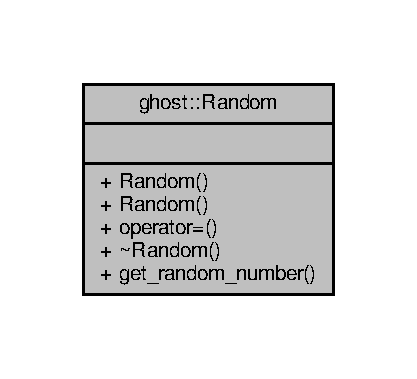
\includegraphics[width=200pt]{classghost_1_1Random__coll__graph}
\end{center}
\end{figure}
\subsection*{Public Member Functions}
\begin{DoxyCompactItemize}
\item 
\hyperlink{classghost_1_1Random_a7c45efd1f7c522a68760104ba6084d89}{Random} ()
\begin{DoxyCompactList}\small\item\em Unique construtor. \end{DoxyCompactList}\item 
\hyperlink{classghost_1_1Random_aa57a39ee45a9ba30d7f7ea2c4c17b539}{Random} (const \hyperlink{classghost_1_1Random}{Random} \&other)
\begin{DoxyCompactList}\small\item\em Unique copy constructor. \end{DoxyCompactList}\item 
\hyperlink{classghost_1_1Random}{Random} \& \hyperlink{classghost_1_1Random_ab9257479f8e393fc8d205f6a05357ee6}{operator=} (\hyperlink{classghost_1_1Random}{Random} other)
\begin{DoxyCompactList}\small\item\em Copy assignment operator following the copy-\/and-\/swap idiom. \end{DoxyCompactList}\item 
\hyperlink{classghost_1_1Random_a5b2a324a97684d12174a6f97bdb43aaa}{$\sim$\+Random} ()=default
\begin{DoxyCompactList}\small\item\em Default destructor. \end{DoxyCompactList}\item 
int \hyperlink{classghost_1_1Random_acc4f1a79621ed8d77c303cecda571034}{get\+\_\+random\+\_\+number} (int limit) const 
\end{DoxyCompactItemize}


\subsection{Detailed Description}
\hyperlink{classghost_1_1Random}{Random} uses the C++11 Mersenne Twister (mt19937) as a pseudo-\/random generator. Seeds are generated by C++11 random\+\_\+device.

It follows a near-\/uniform distribution, but not a uniform one. This is to make the class more convenient to use by creating one \hyperlink{classghost_1_1Random}{Random} object to get numbers within different ranges, instead of forcing creating one \hyperlink{classghost_1_1Random}{Random} object for each specific range. If you need to sample numbers from a purely uniform distribution, do not use this class. 

\subsection{Constructor \& Destructor Documentation}
\index{ghost\+::\+Random@{ghost\+::\+Random}!Random@{Random}}
\index{Random@{Random}!ghost\+::\+Random@{ghost\+::\+Random}}
\subsubsection[{\texorpdfstring{Random()}{Random()}}]{\setlength{\rightskip}{0pt plus 5cm}ghost\+::\+Random\+::\+Random (
\begin{DoxyParamCaption}
{}
\end{DoxyParamCaption}
)\hspace{0.3cm}{\ttfamily [inline]}}\hypertarget{classghost_1_1Random_a7c45efd1f7c522a68760104ba6084d89}{}\label{classghost_1_1Random_a7c45efd1f7c522a68760104ba6084d89}


Unique construtor. 

\index{ghost\+::\+Random@{ghost\+::\+Random}!Random@{Random}}
\index{Random@{Random}!ghost\+::\+Random@{ghost\+::\+Random}}
\subsubsection[{\texorpdfstring{Random(const Random \&other)}{Random(const Random &other)}}]{\setlength{\rightskip}{0pt plus 5cm}ghost\+::\+Random\+::\+Random (
\begin{DoxyParamCaption}
\item[{const {\bf Random} \&}]{other}
\end{DoxyParamCaption}
)\hspace{0.3cm}{\ttfamily [inline]}}\hypertarget{classghost_1_1Random_aa57a39ee45a9ba30d7f7ea2c4c17b539}{}\label{classghost_1_1Random_aa57a39ee45a9ba30d7f7ea2c4c17b539}


Unique copy constructor. 

\index{ghost\+::\+Random@{ghost\+::\+Random}!````~Random@{$\sim$\+Random}}
\index{````~Random@{$\sim$\+Random}!ghost\+::\+Random@{ghost\+::\+Random}}
\subsubsection[{\texorpdfstring{$\sim$\+Random()=default}{~Random()=default}}]{\setlength{\rightskip}{0pt plus 5cm}ghost\+::\+Random\+::$\sim$\+Random (
\begin{DoxyParamCaption}
{}
\end{DoxyParamCaption}
)\hspace{0.3cm}{\ttfamily [default]}}\hypertarget{classghost_1_1Random_a5b2a324a97684d12174a6f97bdb43aaa}{}\label{classghost_1_1Random_a5b2a324a97684d12174a6f97bdb43aaa}


Default destructor. 



\subsection{Member Function Documentation}
\index{ghost\+::\+Random@{ghost\+::\+Random}!get\+\_\+random\+\_\+number@{get\+\_\+random\+\_\+number}}
\index{get\+\_\+random\+\_\+number@{get\+\_\+random\+\_\+number}!ghost\+::\+Random@{ghost\+::\+Random}}
\subsubsection[{\texorpdfstring{get\+\_\+random\+\_\+number(int limit) const }{get_random_number(int limit) const }}]{\setlength{\rightskip}{0pt plus 5cm}int ghost\+::\+Random\+::get\+\_\+random\+\_\+number (
\begin{DoxyParamCaption}
\item[{int}]{limit}
\end{DoxyParamCaption}
) const\hspace{0.3cm}{\ttfamily [inline]}}\hypertarget{classghost_1_1Random_acc4f1a79621ed8d77c303cecda571034}{}\label{classghost_1_1Random_acc4f1a79621ed8d77c303cecda571034}
Inline function returning a pseudo-\/random value from the range \mbox{[}0, limit\mbox{[}, according a near-\/uniform distribution, like discussed above.


\begin{DoxyParams}{Parameters}
{\em limit} & The upper bound of the range \mbox{[}0, limit\mbox{[} from where a random value is computed. \\
\hline
\end{DoxyParams}
\begin{DoxyReturn}{Returns}
A pseudo-\/random value in the range \mbox{[}0, limit\mbox{[} 
\end{DoxyReturn}
\index{ghost\+::\+Random@{ghost\+::\+Random}!operator=@{operator=}}
\index{operator=@{operator=}!ghost\+::\+Random@{ghost\+::\+Random}}
\subsubsection[{\texorpdfstring{operator=(\+Random other)}{operator=(Random other)}}]{\setlength{\rightskip}{0pt plus 5cm}{\bf Random}\& ghost\+::\+Random\+::operator= (
\begin{DoxyParamCaption}
\item[{{\bf Random}}]{other}
\end{DoxyParamCaption}
)\hspace{0.3cm}{\ttfamily [inline]}}\hypertarget{classghost_1_1Random_ab9257479f8e393fc8d205f6a05357ee6}{}\label{classghost_1_1Random_ab9257479f8e393fc8d205f6a05357ee6}


Copy assignment operator following the copy-\/and-\/swap idiom. 



The documentation for this class was generated from the following file\+:\begin{DoxyCompactItemize}
\item 
include/misc/\hyperlink{random_8hpp}{random.\+hpp}\end{DoxyCompactItemize}

\hypertarget{classghost_1_1Solver}{}\section{ghost\+:\+:Solver$<$ Type\+Variable, Type\+Constraint $>$ Class Template Reference}
\label{classghost_1_1Solver}\index{ghost\+::\+Solver$<$ Type\+Variable, Type\+Constraint $>$@{ghost\+::\+Solver$<$ Type\+Variable, Type\+Constraint $>$}}


\hyperlink{classghost_1_1Solver}{Solver} is the class coding the solver itself.  




{\ttfamily \#include $<$solver.\+hpp$>$}



Collaboration diagram for ghost\+:\+:Solver$<$ Type\+Variable, Type\+Constraint $>$\+:\nopagebreak
\begin{figure}[H]
\begin{center}
\leavevmode
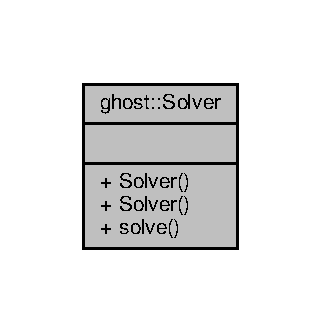
\includegraphics[width=223pt]{classghost_1_1Solver__coll__graph}
\end{center}
\end{figure}
\subsection*{Public Member Functions}
\begin{DoxyCompactItemize}
\item 
\hyperlink{classghost_1_1Solver_afcafbb540e963da0aa0d8bbf5634f6e4}{Solver} (vector$<$ Type\+Variable $>$ \&vec\+Variables, vector$<$ shared\+\_\+ptr$<$ Type\+Constraint $>$$>$ \&vec\+Constraints, shared\+\_\+ptr$<$ \hyperlink{classghost_1_1Objective}{Objective}$<$ Type\+Variable $>$$>$ objecive, bool permutation\+Problem=false)
\begin{DoxyCompactList}\small\item\em \hyperlink{classghost_1_1Solver}{Solver}\textquotesingle{}s regular constructor. \end{DoxyCompactList}\item 
\hyperlink{classghost_1_1Solver_a26fe2a7362fdc6cc44b07e0c658250de}{Solver} (vector$<$ Type\+Variable $>$ \&vec\+Variables, vector$<$ shared\+\_\+ptr$<$ Type\+Constraint $>$$>$ \&vec\+Constraints, bool permutation\+Problem=false)
\begin{DoxyCompactList}\small\item\em Second \hyperlink{classghost_1_1Solver}{Solver}\textquotesingle{}s constructor. \end{DoxyCompactList}\item 
bool \hyperlink{classghost_1_1Solver_ab2f3b79560cefbe8299583a40edad40e}{solve} (double \&final\+Cost, vector$<$ int $>$ \&final\+Solution, double sat\+\_\+timeout, double opt\+\_\+timeout=0.)
\begin{DoxyCompactList}\small\item\em \hyperlink{classghost_1_1Solver}{Solver}\textquotesingle{}s main function, to solve the given C\+S\+P/\+C\+OP. \end{DoxyCompactList}\end{DoxyCompactItemize}


\subsection{Detailed Description}
\subsubsection*{template$<$typename Type\+Variable, typename Type\+Constraint$>$\\*
class ghost\+::\+Solver$<$ Type\+Variable, Type\+Constraint $>$}

\hyperlink{classghost_1_1Solver}{Solver} is the class coding the solver itself. 

You just need to instanciate one \hyperlink{classghost_1_1Solver}{Solver} object, then run its \textquotesingle{}solve\textquotesingle{} function.

The \hyperlink{classghost_1_1Solver}{Solver} class is a template class, waiting for both the type of variable and the type of constraint. Thus, you must instanciate a solver by specifying the class of your variable objects and the class of your constraint objects, like for instance \hyperlink{classghost_1_1Solver}{Solver}$<$My\+Custom\+Variable, My\+Custom\+Constraint$>$ where My\+Custom\+Variable must inherits from \hyperlink{classghost_1_1Variable}{ghost\+::\+Variable} and My\+Custom\+Constraint must inherits from \hyperlink{classghost_1_1Constraint}{ghost\+::\+Constraint}.

Each variable modelling a problem must instanciate the same class. However, constraints of different type can exist within the same problem model. This is the reson why the vector of constraints is a vector of (shared) pointers of \hyperlink{classghost_1_1Constraint}{Constraint}.

\hyperlink{classghost_1_1Solver}{Solver}\textquotesingle{}s constructor also need a shared pointer of an \hyperlink{classghost_1_1Objective}{Objective} object. The reason why \hyperlink{classghost_1_1Objective}{Objective} is not a template parameter of \hyperlink{classghost_1_1Solver}{Solver} but a pointer is to allow a dynamic modification of the objective function.

\begin{DoxySeeAlso}{See also}
\hyperlink{classghost_1_1Variable}{Variable}, \hyperlink{classghost_1_1Constraint}{Constraint}, \hyperlink{classghost_1_1Objective}{Objective} 
\end{DoxySeeAlso}


\subsection{Constructor \& Destructor Documentation}
\index{ghost\+::\+Solver@{ghost\+::\+Solver}!Solver@{Solver}}
\index{Solver@{Solver}!ghost\+::\+Solver@{ghost\+::\+Solver}}
\subsubsection[{\texorpdfstring{Solver(vector$<$ Type\+Variable $>$ \&vec\+Variables, vector$<$ shared\+\_\+ptr$<$ Type\+Constraint $>$$>$ \&vec\+Constraints, shared\+\_\+ptr$<$ Objective$<$ Type\+Variable $>$$>$ objecive, bool permutation\+Problem=false)}{Solver(vector< TypeVariable > &vecVariables, vector< shared_ptr< TypeConstraint >> &vecConstraints, shared_ptr< Objective< TypeVariable >> objecive, bool permutationProblem=false)}}]{\setlength{\rightskip}{0pt plus 5cm}template$<$typename Type\+Variable , typename Type\+Constraint $>$ {\bf ghost\+::\+Solver}$<$ Type\+Variable, Type\+Constraint $>$\+::{\bf Solver} (
\begin{DoxyParamCaption}
\item[{vector$<$ Type\+Variable $>$ \&}]{vec\+Variables, }
\item[{vector$<$ shared\+\_\+ptr$<$ Type\+Constraint $>$$>$ \&}]{vec\+Constraints, }
\item[{shared\+\_\+ptr$<$ {\bf Objective}$<$ Type\+Variable $>$$>$}]{objecive, }
\item[{bool}]{permutation\+Problem = {\ttfamily false}}
\end{DoxyParamCaption}
)}\hypertarget{classghost_1_1Solver_afcafbb540e963da0aa0d8bbf5634f6e4}{}\label{classghost_1_1Solver_afcafbb540e963da0aa0d8bbf5634f6e4}


\hyperlink{classghost_1_1Solver}{Solver}\textquotesingle{}s regular constructor. 


\begin{DoxyParams}{Parameters}
{\em vec\+Variables} & A pointer to the vector of Variables. \\
\hline
{\em vec\+Constraints} & A reference to the vector of Constraints. \\
\hline
{\em obj} & A shared pointer to the \hyperlink{classghost_1_1Objective}{Objective}. \\
\hline
{\em permutation\+Problem} & A boolean indicating if we work on a permutation problem. False by default. \\
\hline
\end{DoxyParams}
\index{ghost\+::\+Solver@{ghost\+::\+Solver}!Solver@{Solver}}
\index{Solver@{Solver}!ghost\+::\+Solver@{ghost\+::\+Solver}}
\subsubsection[{\texorpdfstring{Solver(vector$<$ Type\+Variable $>$ \&vec\+Variables, vector$<$ shared\+\_\+ptr$<$ Type\+Constraint $>$$>$ \&vec\+Constraints, bool permutation\+Problem=false)}{Solver(vector< TypeVariable > &vecVariables, vector< shared_ptr< TypeConstraint >> &vecConstraints, bool permutationProblem=false)}}]{\setlength{\rightskip}{0pt plus 5cm}template$<$typename Type\+Variable , typename Type\+Constraint $>$ {\bf ghost\+::\+Solver}$<$ Type\+Variable, Type\+Constraint $>$\+::{\bf Solver} (
\begin{DoxyParamCaption}
\item[{vector$<$ Type\+Variable $>$ \&}]{vec\+Variables, }
\item[{vector$<$ shared\+\_\+ptr$<$ Type\+Constraint $>$$>$ \&}]{vec\+Constraints, }
\item[{bool}]{permutation\+Problem = {\ttfamily false}}
\end{DoxyParamCaption}
)}\hypertarget{classghost_1_1Solver_a26fe2a7362fdc6cc44b07e0c658250de}{}\label{classghost_1_1Solver_a26fe2a7362fdc6cc44b07e0c658250de}


Second \hyperlink{classghost_1_1Solver}{Solver}\textquotesingle{}s constructor. 


\begin{DoxyParams}{Parameters}
{\em vec\+Variables} & A reference to the vector of Variables. \\
\hline
{\em vec\+Constraints} & A reference to the vector of Constraints. \\
\hline
{\em permutation\+Problem} & A boolean indicating if we work on a permutation problem. False by default. \\
\hline
\end{DoxyParams}


\subsection{Member Function Documentation}
\index{ghost\+::\+Solver@{ghost\+::\+Solver}!solve@{solve}}
\index{solve@{solve}!ghost\+::\+Solver@{ghost\+::\+Solver}}
\subsubsection[{\texorpdfstring{solve(double \&final\+Cost, vector$<$ int $>$ \&final\+Solution, double sat\+\_\+timeout, double opt\+\_\+timeout=0.)}{solve(double &finalCost, vector< int > &finalSolution, double sat_timeout, double opt_timeout=0.)}}]{\setlength{\rightskip}{0pt plus 5cm}template$<$typename Type\+Variable , typename Type\+Constraint $>$ bool {\bf ghost\+::\+Solver}$<$ Type\+Variable, Type\+Constraint $>$\+::solve (
\begin{DoxyParamCaption}
\item[{double \&}]{final\+Cost, }
\item[{vector$<$ int $>$ \&}]{final\+Solution, }
\item[{double}]{sat\+\_\+timeout, }
\item[{double}]{opt\+\_\+timeout = {\ttfamily 0.}}
\end{DoxyParamCaption}
)}\hypertarget{classghost_1_1Solver_ab2f3b79560cefbe8299583a40edad40e}{}\label{classghost_1_1Solver_ab2f3b79560cefbe8299583a40edad40e}


\hyperlink{classghost_1_1Solver}{Solver}\textquotesingle{}s main function, to solve the given C\+S\+P/\+C\+OP. 


\begin{DoxyParams}{Parameters}
{\em final\+Cost} & A reference to the double of the sum of constraints cost for satisfaction problems, or the value of the objective function for optimization problems. For satisfaction problems, a cost of zero means a solution has been found. \\
\hline
{\em final\+Solution} & The configuration of the best solution found, ie, a reference to the vector of assignements of each variable. \\
\hline
{\em sat\+\_\+timeout} & The satisfaction timeout in milliseconds. \\
\hline
{\em opt\+\_\+timeout} & The optimization timeout in milliseconds (optionnal, equals to 10 times sat\+\_\+timeout is not set). \\
\hline
\end{DoxyParams}
\begin{DoxyReturn}{Returns}
True iff a solution has been found. 
\end{DoxyReturn}


The documentation for this class was generated from the following file\+:\begin{DoxyCompactItemize}
\item 
include/\hyperlink{solver_8hpp}{solver.\+hpp}\end{DoxyCompactItemize}

\hypertarget{classghost_1_1Variable}{}\section{ghost\+:\+:Variable Class Reference}
\label{classghost_1_1Variable}\index{ghost\+::\+Variable@{ghost\+::\+Variable}}


\hyperlink{classghost_1_1Variable}{Variable} is the class encoding the variables of your C\+S\+P/\+C\+OP.  




{\ttfamily \#include $<$variable.\+hpp$>$}



Collaboration diagram for ghost\+:\+:Variable\+:
\nopagebreak
\begin{figure}[H]
\begin{center}
\leavevmode
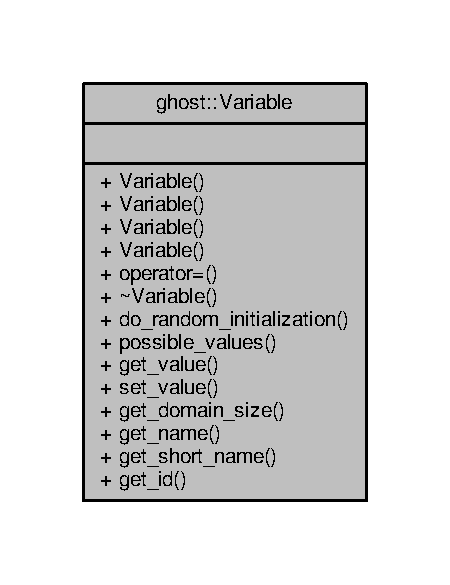
\includegraphics[width=216pt]{classghost_1_1Variable__coll__graph}
\end{center}
\end{figure}
\subsection*{Public Member Functions}
\begin{DoxyCompactItemize}
\item 
\hyperlink{classghost_1_1Variable_a41d27734b85f60c2e5fda7ee0ab5c600}{Variable} ()=delete
\begin{DoxyCompactList}\small\item\em The default \hyperlink{classghost_1_1Variable}{Variable} constructor is disabled. \end{DoxyCompactList}\item 
\hyperlink{classghost_1_1Variable_aa5dc881b8a239206bf55d018cc4a2156}{Variable} (const string \&\hyperlink{classghost_1_1Variable_a05cf4a4cd3a5c033028e0b0f11d1dafd}{name}, const string \&\hyperlink{classghost_1_1Variable_afb5eb79a7f6351b4305fe082699b6d7d}{short\+Name}, const vector$<$ int $>$ \&\hyperlink{classghost_1_1Variable_ab3d7bfa2e8c2139473775a6b797d0991}{domain}, int \hyperlink{classghost_1_1Variable_a934efa463fb1897b4266040e321dbc41}{index}=0)
\begin{DoxyCompactList}\small\item\em First \hyperlink{classghost_1_1Variable}{Variable} constructor, with the vector of domain values and the outside-\/the-\/scope value. \end{DoxyCompactList}\item 
\hyperlink{classghost_1_1Variable_a98be1149bd927b36a7914756641d6196}{Variable} (const string \&\hyperlink{classghost_1_1Variable_a05cf4a4cd3a5c033028e0b0f11d1dafd}{name}, const string \&\hyperlink{classghost_1_1Variable_afb5eb79a7f6351b4305fe082699b6d7d}{short\+Name}, int size, int start\+Value, int \hyperlink{classghost_1_1Variable_a934efa463fb1897b4266040e321dbc41}{index}=0)
\begin{DoxyCompactList}\small\item\em Second \hyperlink{classghost_1_1Variable}{Variable} constructor, with a size and a starting value for the domain. \end{DoxyCompactList}\item 
\hyperlink{classghost_1_1Variable_ac9fb0513e1d15a047816821e034589ea}{Variable} (const \hyperlink{classghost_1_1Variable}{Variable} \&other)
\begin{DoxyCompactList}\small\item\em \hyperlink{classghost_1_1Variable}{Variable} copy constructor. \end{DoxyCompactList}\item 
\hyperlink{classghost_1_1Variable}{Variable} \& \hyperlink{classghost_1_1Variable_ad82b892892c3531cc3d54d6b5d048bf6}{operator=} (\hyperlink{classghost_1_1Variable}{Variable} other)
\begin{DoxyCompactList}\small\item\em \hyperlink{classghost_1_1Variable}{Variable}\textquotesingle{}s copy assignment operator. \end{DoxyCompactList}\item 
virtual \hyperlink{classghost_1_1Variable_a718686ab389bd31ae0f3cbb312c9be77}{$\sim$\+Variable} ()=default
\begin{DoxyCompactList}\small\item\em Default \hyperlink{classghost_1_1Variable}{Variable} destructor. \end{DoxyCompactList}\item 
void \hyperlink{classghost_1_1Variable_a37018e24ee21e12649599409d7ac3640}{do\+\_\+random\+\_\+initialization} ()
\begin{DoxyCompactList}\small\item\em Function initializing the variable to one random values of its domain. \end{DoxyCompactList}\item 
const vector$<$ int $>$ \& \hyperlink{classghost_1_1Variable_a82380b5d0d4f679401c0139d5d30ad60}{possible\+\_\+values} () const 
\item 
int \hyperlink{classghost_1_1Variable_a7bdebf8b2a369f337690ac38ece31793}{get\+\_\+value} () const 
\begin{DoxyCompactList}\small\item\em Inline function to get the current value of the variable. \end{DoxyCompactList}\item 
void \hyperlink{classghost_1_1Variable_a06f6c296986a017e1713961b4d763b0c}{set\+\_\+value} (int value)
\begin{DoxyCompactList}\small\item\em Inline function to set the value of the variable. \end{DoxyCompactList}\item 
size\+\_\+t \hyperlink{classghost_1_1Variable_afd4a3fe7e7a6d1438c4e90c72b77eee7}{get\+\_\+domain\+\_\+size} ()
\begin{DoxyCompactList}\small\item\em Inline function returning the size of the domain of the variable. \end{DoxyCompactList}\item 
string \hyperlink{classghost_1_1Variable_a70c22841aa8d0ebe75eea92f1831c126}{get\+\_\+name} () const 
\begin{DoxyCompactList}\small\item\em Inline function to get the variable name. \end{DoxyCompactList}\item 
string \hyperlink{classghost_1_1Variable_a993e65196f2bcd0e5e5f4453736e36c5}{get\+\_\+short\+\_\+name} () const 
\begin{DoxyCompactList}\small\item\em Inline function to get the variable short name. \end{DoxyCompactList}\item 
int \hyperlink{classghost_1_1Variable_adc5da5dedaa3d47a5eb4092b08c3f77c}{get\+\_\+id} () const 
\begin{DoxyCompactList}\small\item\em Inline function to get the unique id of the \hyperlink{classghost_1_1Variable}{Variable} object. \end{DoxyCompactList}\end{DoxyCompactItemize}
\subsection*{Protected Attributes}
\begin{DoxyCompactItemize}
\item 
string \hyperlink{classghost_1_1Variable_a05cf4a4cd3a5c033028e0b0f11d1dafd}{name}
\begin{DoxyCompactList}\small\item\em A string to give a full name to the variable (for instance, \char`\"{}\+Barracks\char`\"{}). \end{DoxyCompactList}\item 
string \hyperlink{classghost_1_1Variable_afb5eb79a7f6351b4305fe082699b6d7d}{short\+Name}
\begin{DoxyCompactList}\small\item\em A string to give a shorten name to the variable (for instance, \char`\"{}\+B\char`\"{}). \end{DoxyCompactList}\item 
\hyperlink{classghost_1_1Domain}{Domain} \hyperlink{classghost_1_1Variable_ab3d7bfa2e8c2139473775a6b797d0991}{domain}
\begin{DoxyCompactList}\small\item\em The domain of the variable. \end{DoxyCompactList}\item 
int \hyperlink{classghost_1_1Variable_a934efa463fb1897b4266040e321dbc41}{index}
\begin{DoxyCompactList}\small\item\em The domain\textquotesingle{}s index corresponding to the current value of the variable. \end{DoxyCompactList}\end{DoxyCompactItemize}
\subsection*{Friends}
\begin{DoxyCompactItemize}
\item 
ostream \& \hyperlink{classghost_1_1Variable_af674a590cfa8082686f61b22cbb15790}{operator$<$$<$} (ostream \&os, const \hyperlink{classghost_1_1Variable}{Variable} \&v)
\end{DoxyCompactItemize}


\subsection{Detailed Description}
\hyperlink{classghost_1_1Variable}{Variable} is the class encoding the variables of your C\+S\+P/\+C\+OP. 

In G\+H\+O\+ST, all variable objects must be instanciate from the same concrete class. Be careful to model your C\+S\+P/\+C\+OP in order to use one kind of variable only, ie., all variable objects in the implementation of your C\+S\+P/\+C\+OP must be instanciated from the same \hyperlink{classghost_1_1Variable}{Variable} (sub)class.

To encode your C\+S\+P/\+C\+OP variables, you can either directly use this class \hyperlink{classghost_1_1Variable}{Variable} (there are no pure virtual functions here), or inherit from it to make your own variable class.

\begin{DoxySeeAlso}{See also}
\hyperlink{classghost_1_1Domain}{Domain} 
\end{DoxySeeAlso}


\subsection{Constructor \& Destructor Documentation}
\index{ghost\+::\+Variable@{ghost\+::\+Variable}!Variable@{Variable}}
\index{Variable@{Variable}!ghost\+::\+Variable@{ghost\+::\+Variable}}
\subsubsection[{\texorpdfstring{Variable()=delete}{Variable()=delete}}]{\setlength{\rightskip}{0pt plus 5cm}ghost\+::\+Variable\+::\+Variable (
\begin{DoxyParamCaption}
{}
\end{DoxyParamCaption}
)\hspace{0.3cm}{\ttfamily [delete]}}\hypertarget{classghost_1_1Variable_a41d27734b85f60c2e5fda7ee0ab5c600}{}\label{classghost_1_1Variable_a41d27734b85f60c2e5fda7ee0ab5c600}


The default \hyperlink{classghost_1_1Variable}{Variable} constructor is disabled. 

\index{ghost\+::\+Variable@{ghost\+::\+Variable}!Variable@{Variable}}
\index{Variable@{Variable}!ghost\+::\+Variable@{ghost\+::\+Variable}}
\subsubsection[{\texorpdfstring{Variable(const string \&name, const string \&short\+Name, const vector$<$ int $>$ \&domain, int index=0)}{Variable(const string &name, const string &shortName, const vector< int > &domain, int index=0)}}]{\setlength{\rightskip}{0pt plus 5cm}ghost\+::\+Variable\+::\+Variable (
\begin{DoxyParamCaption}
\item[{const string \&}]{name, }
\item[{const string \&}]{short\+Name, }
\item[{const vector$<$ int $>$ \&}]{domain, }
\item[{int}]{index = {\ttfamily 0}}
\end{DoxyParamCaption}
)}\hypertarget{classghost_1_1Variable_aa5dc881b8a239206bf55d018cc4a2156}{}\label{classghost_1_1Variable_aa5dc881b8a239206bf55d018cc4a2156}


First \hyperlink{classghost_1_1Variable}{Variable} constructor, with the vector of domain values and the outside-\/the-\/scope value. 


\begin{DoxyParams}{Parameters}
{\em name} & A const reference of a string to give a full name to the variable (for instance, \char`\"{}\+Barracks\char`\"{}). \\
\hline
{\em short\+Name} & A const reference of a string to give a shorten name to the variable (for instance, \char`\"{}\+B\char`\"{}). \\
\hline
{\em domain} & A const reference to the vector of integers composing the domain to create. \\
\hline
{\em index} & The domain\textquotesingle{}s index corresponding to the variable initial value. Zero by default. \\
\hline
\end{DoxyParams}
\index{ghost\+::\+Variable@{ghost\+::\+Variable}!Variable@{Variable}}
\index{Variable@{Variable}!ghost\+::\+Variable@{ghost\+::\+Variable}}
\subsubsection[{\texorpdfstring{Variable(const string \&name, const string \&short\+Name, int size, int start\+Value, int index=0)}{Variable(const string &name, const string &shortName, int size, int startValue, int index=0)}}]{\setlength{\rightskip}{0pt plus 5cm}ghost\+::\+Variable\+::\+Variable (
\begin{DoxyParamCaption}
\item[{const string \&}]{name, }
\item[{const string \&}]{short\+Name, }
\item[{int}]{size, }
\item[{int}]{start\+Value, }
\item[{int}]{index = {\ttfamily 0}}
\end{DoxyParamCaption}
)}\hypertarget{classghost_1_1Variable_a98be1149bd927b36a7914756641d6196}{}\label{classghost_1_1Variable_a98be1149bd927b36a7914756641d6196}


Second \hyperlink{classghost_1_1Variable}{Variable} constructor, with a size and a starting value for the domain. 


\begin{DoxyParams}{Parameters}
{\em name} & A const reference of a string to give a full name to the variable (for instance, \char`\"{}\+Barracks\char`\"{}). \\
\hline
{\em short\+Name} & A const reference of a string to give a shorten name to the variable (for instance, \char`\"{}\+B\char`\"{}). \\
\hline
{\em size} & The size of the domain to create. \\
\hline
{\em start\+Value} & An integer representing the first value of the domain. The creating domain will then be the interval \mbox{[}start\+Value, start\+Value + size\mbox{]}. \\
\hline
{\em index} & The domain\textquotesingle{}s index corresponding to the variable initial value. Zero by default. \\
\hline
\end{DoxyParams}
\index{ghost\+::\+Variable@{ghost\+::\+Variable}!Variable@{Variable}}
\index{Variable@{Variable}!ghost\+::\+Variable@{ghost\+::\+Variable}}
\subsubsection[{\texorpdfstring{Variable(const Variable \&other)}{Variable(const Variable &other)}}]{\setlength{\rightskip}{0pt plus 5cm}ghost\+::\+Variable\+::\+Variable (
\begin{DoxyParamCaption}
\item[{const {\bf Variable} \&}]{other}
\end{DoxyParamCaption}
)}\hypertarget{classghost_1_1Variable_ac9fb0513e1d15a047816821e034589ea}{}\label{classghost_1_1Variable_ac9fb0513e1d15a047816821e034589ea}


\hyperlink{classghost_1_1Variable}{Variable} copy constructor. 


\begin{DoxyParams}{Parameters}
{\em other} & A const reference to a \hyperlink{classghost_1_1Variable}{Variable} object. \\
\hline
\end{DoxyParams}
\index{ghost\+::\+Variable@{ghost\+::\+Variable}!````~Variable@{$\sim$\+Variable}}
\index{````~Variable@{$\sim$\+Variable}!ghost\+::\+Variable@{ghost\+::\+Variable}}
\subsubsection[{\texorpdfstring{$\sim$\+Variable()=default}{~Variable()=default}}]{\setlength{\rightskip}{0pt plus 5cm}virtual ghost\+::\+Variable\+::$\sim$\+Variable (
\begin{DoxyParamCaption}
{}
\end{DoxyParamCaption}
)\hspace{0.3cm}{\ttfamily [virtual]}, {\ttfamily [default]}}\hypertarget{classghost_1_1Variable_a718686ab389bd31ae0f3cbb312c9be77}{}\label{classghost_1_1Variable_a718686ab389bd31ae0f3cbb312c9be77}


Default \hyperlink{classghost_1_1Variable}{Variable} destructor. 



\subsection{Member Function Documentation}
\index{ghost\+::\+Variable@{ghost\+::\+Variable}!do\+\_\+random\+\_\+initialization@{do\+\_\+random\+\_\+initialization}}
\index{do\+\_\+random\+\_\+initialization@{do\+\_\+random\+\_\+initialization}!ghost\+::\+Variable@{ghost\+::\+Variable}}
\subsubsection[{\texorpdfstring{do\+\_\+random\+\_\+initialization()}{do_random_initialization()}}]{\setlength{\rightskip}{0pt plus 5cm}void ghost\+::\+Variable\+::do\+\_\+random\+\_\+initialization (
\begin{DoxyParamCaption}
{}
\end{DoxyParamCaption}
)}\hypertarget{classghost_1_1Variable_a37018e24ee21e12649599409d7ac3640}{}\label{classghost_1_1Variable_a37018e24ee21e12649599409d7ac3640}


Function initializing the variable to one random values of its domain. 

\index{ghost\+::\+Variable@{ghost\+::\+Variable}!get\+\_\+domain\+\_\+size@{get\+\_\+domain\+\_\+size}}
\index{get\+\_\+domain\+\_\+size@{get\+\_\+domain\+\_\+size}!ghost\+::\+Variable@{ghost\+::\+Variable}}
\subsubsection[{\texorpdfstring{get\+\_\+domain\+\_\+size()}{get_domain_size()}}]{\setlength{\rightskip}{0pt plus 5cm}size\+\_\+t ghost\+::\+Variable\+::get\+\_\+domain\+\_\+size (
\begin{DoxyParamCaption}
{}
\end{DoxyParamCaption}
)\hspace{0.3cm}{\ttfamily [inline]}}\hypertarget{classghost_1_1Variable_afd4a3fe7e7a6d1438c4e90c72b77eee7}{}\label{classghost_1_1Variable_afd4a3fe7e7a6d1438c4e90c72b77eee7}


Inline function returning the size of the domain of the variable. 

\begin{DoxyReturn}{Returns}
a size\+\_\+t equals to size of the domain of the variable. 
\end{DoxyReturn}
\begin{DoxySeeAlso}{See also}
\hyperlink{classghost_1_1Domain}{Domain} 
\end{DoxySeeAlso}
\index{ghost\+::\+Variable@{ghost\+::\+Variable}!get\+\_\+id@{get\+\_\+id}}
\index{get\+\_\+id@{get\+\_\+id}!ghost\+::\+Variable@{ghost\+::\+Variable}}
\subsubsection[{\texorpdfstring{get\+\_\+id() const }{get_id() const }}]{\setlength{\rightskip}{0pt plus 5cm}int ghost\+::\+Variable\+::get\+\_\+id (
\begin{DoxyParamCaption}
{}
\end{DoxyParamCaption}
) const\hspace{0.3cm}{\ttfamily [inline]}}\hypertarget{classghost_1_1Variable_adc5da5dedaa3d47a5eb4092b08c3f77c}{}\label{classghost_1_1Variable_adc5da5dedaa3d47a5eb4092b08c3f77c}


Inline function to get the unique id of the \hyperlink{classghost_1_1Variable}{Variable} object. 

\index{ghost\+::\+Variable@{ghost\+::\+Variable}!get\+\_\+name@{get\+\_\+name}}
\index{get\+\_\+name@{get\+\_\+name}!ghost\+::\+Variable@{ghost\+::\+Variable}}
\subsubsection[{\texorpdfstring{get\+\_\+name() const }{get_name() const }}]{\setlength{\rightskip}{0pt plus 5cm}string ghost\+::\+Variable\+::get\+\_\+name (
\begin{DoxyParamCaption}
{}
\end{DoxyParamCaption}
) const\hspace{0.3cm}{\ttfamily [inline]}}\hypertarget{classghost_1_1Variable_a70c22841aa8d0ebe75eea92f1831c126}{}\label{classghost_1_1Variable_a70c22841aa8d0ebe75eea92f1831c126}


Inline function to get the variable name. 

\index{ghost\+::\+Variable@{ghost\+::\+Variable}!get\+\_\+short\+\_\+name@{get\+\_\+short\+\_\+name}}
\index{get\+\_\+short\+\_\+name@{get\+\_\+short\+\_\+name}!ghost\+::\+Variable@{ghost\+::\+Variable}}
\subsubsection[{\texorpdfstring{get\+\_\+short\+\_\+name() const }{get_short_name() const }}]{\setlength{\rightskip}{0pt plus 5cm}string ghost\+::\+Variable\+::get\+\_\+short\+\_\+name (
\begin{DoxyParamCaption}
{}
\end{DoxyParamCaption}
) const\hspace{0.3cm}{\ttfamily [inline]}}\hypertarget{classghost_1_1Variable_a993e65196f2bcd0e5e5f4453736e36c5}{}\label{classghost_1_1Variable_a993e65196f2bcd0e5e5f4453736e36c5}


Inline function to get the variable short name. 

\index{ghost\+::\+Variable@{ghost\+::\+Variable}!get\+\_\+value@{get\+\_\+value}}
\index{get\+\_\+value@{get\+\_\+value}!ghost\+::\+Variable@{ghost\+::\+Variable}}
\subsubsection[{\texorpdfstring{get\+\_\+value() const }{get_value() const }}]{\setlength{\rightskip}{0pt plus 5cm}int ghost\+::\+Variable\+::get\+\_\+value (
\begin{DoxyParamCaption}
{}
\end{DoxyParamCaption}
) const\hspace{0.3cm}{\ttfamily [inline]}}\hypertarget{classghost_1_1Variable_a7bdebf8b2a369f337690ac38ece31793}{}\label{classghost_1_1Variable_a7bdebf8b2a369f337690ac38ece31793}


Inline function to get the current value of the variable. 

If the index do not belong to the \hyperlink{classghost_1_1Domain}{Domain} range, raises an index\+Exception. \begin{DoxySeeAlso}{See also}
\hyperlink{classghost_1_1Domain}{Domain} 
\end{DoxySeeAlso}
\index{ghost\+::\+Variable@{ghost\+::\+Variable}!operator=@{operator=}}
\index{operator=@{operator=}!ghost\+::\+Variable@{ghost\+::\+Variable}}
\subsubsection[{\texorpdfstring{operator=(\+Variable other)}{operator=(Variable other)}}]{\setlength{\rightskip}{0pt plus 5cm}{\bf Variable}\& ghost\+::\+Variable\+::operator= (
\begin{DoxyParamCaption}
\item[{{\bf Variable}}]{other}
\end{DoxyParamCaption}
)}\hypertarget{classghost_1_1Variable_ad82b892892c3531cc3d54d6b5d048bf6}{}\label{classghost_1_1Variable_ad82b892892c3531cc3d54d6b5d048bf6}


\hyperlink{classghost_1_1Variable}{Variable}\textquotesingle{}s copy assignment operator. 

The copy-\/and-\/swap idiom is applyed here.


\begin{DoxyParams}{Parameters}
{\em other} & A \hyperlink{classghost_1_1Variable}{Variable} object. \\
\hline
\end{DoxyParams}
\index{ghost\+::\+Variable@{ghost\+::\+Variable}!possible\+\_\+values@{possible\+\_\+values}}
\index{possible\+\_\+values@{possible\+\_\+values}!ghost\+::\+Variable@{ghost\+::\+Variable}}
\subsubsection[{\texorpdfstring{possible\+\_\+values() const }{possible_values() const }}]{\setlength{\rightskip}{0pt plus 5cm}const vector$<$int$>$\& ghost\+::\+Variable\+::possible\+\_\+values (
\begin{DoxyParamCaption}
{}
\end{DoxyParamCaption}
) const}\hypertarget{classghost_1_1Variable_a82380b5d0d4f679401c0139d5d30ad60}{}\label{classghost_1_1Variable_a82380b5d0d4f679401c0139d5d30ad60}
Function returning what values are in the domain. \begin{DoxyReturn}{Returns}
a vector$<$int$>$ of values belonging to the variable domain. 
\end{DoxyReturn}
\index{ghost\+::\+Variable@{ghost\+::\+Variable}!set\+\_\+value@{set\+\_\+value}}
\index{set\+\_\+value@{set\+\_\+value}!ghost\+::\+Variable@{ghost\+::\+Variable}}
\subsubsection[{\texorpdfstring{set\+\_\+value(int value)}{set_value(int value)}}]{\setlength{\rightskip}{0pt plus 5cm}void ghost\+::\+Variable\+::set\+\_\+value (
\begin{DoxyParamCaption}
\item[{int}]{value}
\end{DoxyParamCaption}
)\hspace{0.3cm}{\ttfamily [inline]}}\hypertarget{classghost_1_1Variable_a06f6c296986a017e1713961b4d763b0c}{}\label{classghost_1_1Variable_a06f6c296986a017e1713961b4d763b0c}


Inline function to set the value of the variable. 

If the given value is not in the domain, raises a value\+Exception. 
\begin{DoxyParams}{Parameters}
{\em value} & An integer representing the new value to set. \\
\hline
\end{DoxyParams}
\begin{DoxySeeAlso}{See also}
\hyperlink{classghost_1_1Domain}{Domain} 
\end{DoxySeeAlso}


\subsection{Friends And Related Function Documentation}
\index{ghost\+::\+Variable@{ghost\+::\+Variable}!operator$<$$<$@{operator$<$$<$}}
\index{operator$<$$<$@{operator$<$$<$}!ghost\+::\+Variable@{ghost\+::\+Variable}}
\subsubsection[{\texorpdfstring{operator$<$$<$}{operator<<}}]{\setlength{\rightskip}{0pt plus 5cm}ostream\& operator$<$$<$ (
\begin{DoxyParamCaption}
\item[{ostream \&}]{os, }
\item[{const {\bf Variable} \&}]{v}
\end{DoxyParamCaption}
)\hspace{0.3cm}{\ttfamily [friend]}}\hypertarget{classghost_1_1Variable_af674a590cfa8082686f61b22cbb15790}{}\label{classghost_1_1Variable_af674a590cfa8082686f61b22cbb15790}


\subsection{Member Data Documentation}
\index{ghost\+::\+Variable@{ghost\+::\+Variable}!domain@{domain}}
\index{domain@{domain}!ghost\+::\+Variable@{ghost\+::\+Variable}}
\subsubsection[{\texorpdfstring{domain}{domain}}]{\setlength{\rightskip}{0pt plus 5cm}{\bf Domain} ghost\+::\+Variable\+::domain\hspace{0.3cm}{\ttfamily [protected]}}\hypertarget{classghost_1_1Variable_ab3d7bfa2e8c2139473775a6b797d0991}{}\label{classghost_1_1Variable_ab3d7bfa2e8c2139473775a6b797d0991}


The domain of the variable. 

\index{ghost\+::\+Variable@{ghost\+::\+Variable}!index@{index}}
\index{index@{index}!ghost\+::\+Variable@{ghost\+::\+Variable}}
\subsubsection[{\texorpdfstring{index}{index}}]{\setlength{\rightskip}{0pt plus 5cm}int ghost\+::\+Variable\+::index\hspace{0.3cm}{\ttfamily [protected]}}\hypertarget{classghost_1_1Variable_a934efa463fb1897b4266040e321dbc41}{}\label{classghost_1_1Variable_a934efa463fb1897b4266040e321dbc41}


The domain\textquotesingle{}s index corresponding to the current value of the variable. 

\index{ghost\+::\+Variable@{ghost\+::\+Variable}!name@{name}}
\index{name@{name}!ghost\+::\+Variable@{ghost\+::\+Variable}}
\subsubsection[{\texorpdfstring{name}{name}}]{\setlength{\rightskip}{0pt plus 5cm}string ghost\+::\+Variable\+::name\hspace{0.3cm}{\ttfamily [protected]}}\hypertarget{classghost_1_1Variable_a05cf4a4cd3a5c033028e0b0f11d1dafd}{}\label{classghost_1_1Variable_a05cf4a4cd3a5c033028e0b0f11d1dafd}


A string to give a full name to the variable (for instance, \char`\"{}\+Barracks\char`\"{}). 

\index{ghost\+::\+Variable@{ghost\+::\+Variable}!short\+Name@{short\+Name}}
\index{short\+Name@{short\+Name}!ghost\+::\+Variable@{ghost\+::\+Variable}}
\subsubsection[{\texorpdfstring{short\+Name}{shortName}}]{\setlength{\rightskip}{0pt plus 5cm}string ghost\+::\+Variable\+::short\+Name\hspace{0.3cm}{\ttfamily [protected]}}\hypertarget{classghost_1_1Variable_afb5eb79a7f6351b4305fe082699b6d7d}{}\label{classghost_1_1Variable_afb5eb79a7f6351b4305fe082699b6d7d}


A string to give a shorten name to the variable (for instance, \char`\"{}\+B\char`\"{}). 



The documentation for this class was generated from the following file\+:\begin{DoxyCompactItemize}
\item 
include/\hyperlink{variable_8hpp}{variable.\+hpp}\end{DoxyCompactItemize}

\chapter{File Documentation}
\hypertarget{mainpage_8dox}{\section{doc/mainpage.dox File Reference}
\label{mainpage_8dox}\index{doc/mainpage.\-dox@{doc/mainpage.\-dox}}
}

\hypertarget{constraint_8hpp}{\section{include/constraint.hpp File Reference}
\label{constraint_8hpp}\index{include/constraint.\-hpp@{include/constraint.\-hpp}}
}
{\ttfamily \#include $<$vector$>$}\\*
{\ttfamily \#include $<$iostream$>$}\\*
{\ttfamily \#include $<$memory$>$}\\*
{\ttfamily \#include $<$typeinfo$>$}\\*
{\ttfamily \#include \char`\"{}variable.\-hpp\char`\"{}}\\*
Include dependency graph for constraint.\-hpp\-:\nopagebreak
\begin{figure}[H]
\begin{center}
\leavevmode
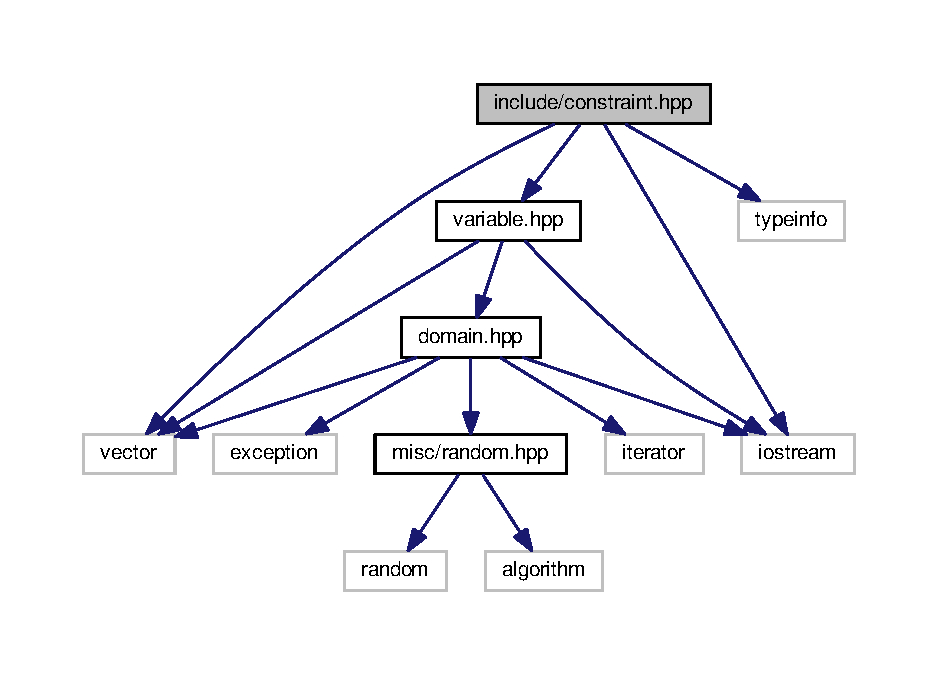
\includegraphics[width=350pt]{constraint_8hpp__incl}
\end{center}
\end{figure}
This graph shows which files directly or indirectly include this file\-:\nopagebreak
\begin{figure}[H]
\begin{center}
\leavevmode
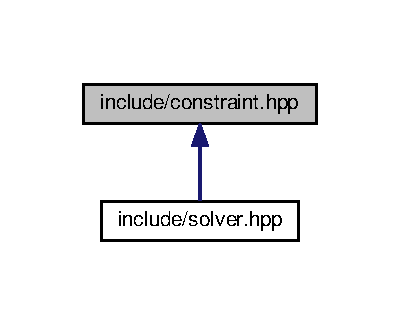
\includegraphics[width=190pt]{constraint_8hpp__dep__incl}
\end{center}
\end{figure}
\subsection*{Classes}
\begin{DoxyCompactItemize}
\item 
class \hyperlink{classghost_1_1Constraint}{ghost\-::\-Constraint}
\begin{DoxyCompactList}\small\item\em \hyperlink{classghost_1_1Constraint}{Constraint} is the class encoding constraints of your C\-S\-P/\-C\-O\-P. \end{DoxyCompactList}\end{DoxyCompactItemize}
\subsection*{Namespaces}
\begin{DoxyCompactItemize}
\item 
\hyperlink{namespaceghost}{ghost}
\end{DoxyCompactItemize}

\hypertarget{domain_8hpp}{\section{include/domain.hpp File Reference}
\label{domain_8hpp}\index{include/domain.\-hpp@{include/domain.\-hpp}}
}
{\ttfamily \#include $<$vector$>$}\\*
{\ttfamily \#include $<$iostream$>$}\\*
{\ttfamily \#include $<$typeinfo$>$}\\*
{\ttfamily \#include $<$algorithm$>$}\\*
{\ttfamily \#include $<$numeric$>$}\\*
{\ttfamily \#include $<$iterator$>$}\\*
{\ttfamily \#include $<$exception$>$}\\*
{\ttfamily \#include \char`\"{}misc/random.\-hpp\char`\"{}}\\*
Include dependency graph for domain.\-hpp\-:
\nopagebreak
\begin{figure}[H]
\begin{center}
\leavevmode
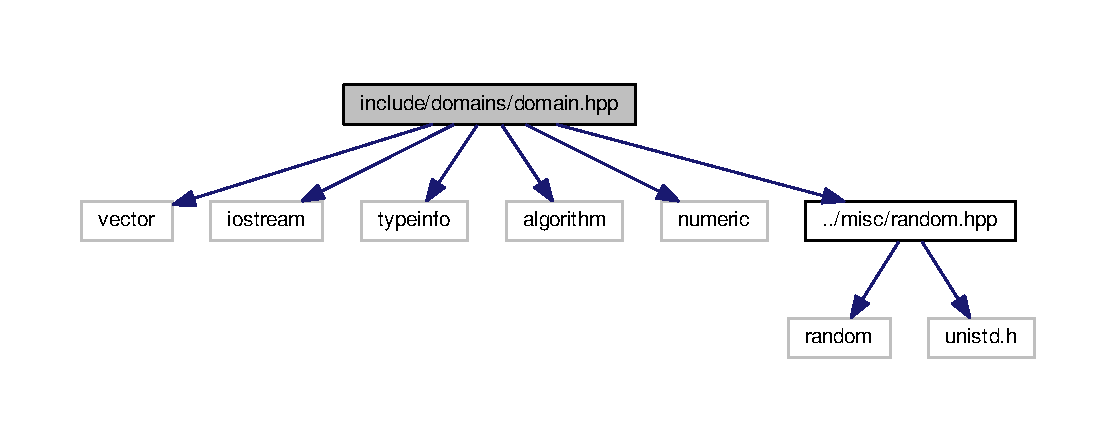
\includegraphics[width=350pt]{domain_8hpp__incl}
\end{center}
\end{figure}
This graph shows which files directly or indirectly include this file\-:
\nopagebreak
\begin{figure}[H]
\begin{center}
\leavevmode
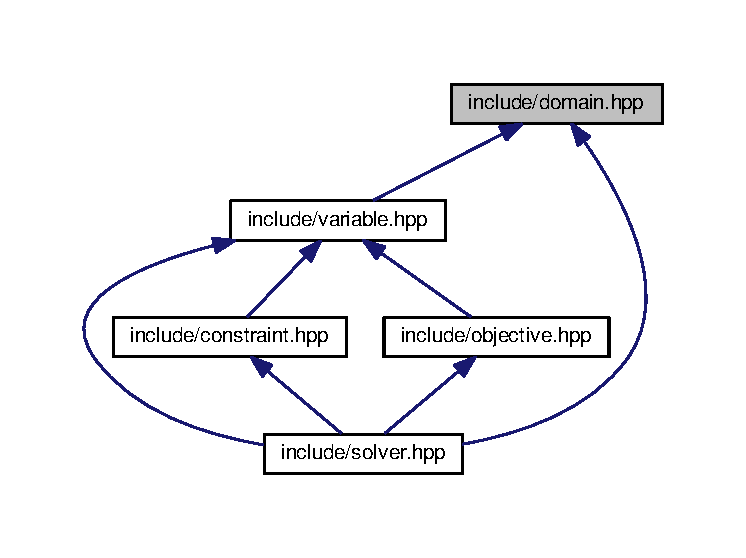
\includegraphics[width=180pt]{domain_8hpp__dep__incl}
\end{center}
\end{figure}
\subsection*{Classes}
\begin{DoxyCompactItemize}
\item 
class \hyperlink{classghost_1_1Domain}{ghost\-::\-Domain}
\begin{DoxyCompactList}\small\item\em \hyperlink{classghost_1_1Domain}{Domain} is the class encoding the domain of your C\-S\-P/\-C\-O\-P. \end{DoxyCompactList}\end{DoxyCompactItemize}
\subsection*{Namespaces}
\begin{DoxyCompactItemize}
\item 
\hyperlink{namespaceghost}{ghost}
\end{DoxyCompactItemize}

\hypertarget{random_8hpp}{\section{include/misc/random.hpp File Reference}
\label{random_8hpp}\index{include/misc/random.\-hpp@{include/misc/random.\-hpp}}
}
{\ttfamily \#include $<$random$>$}\\*
{\ttfamily \#include $<$unistd.\-h$>$}\\*
Include dependency graph for random.\-hpp\-:\nopagebreak
\begin{figure}[H]
\begin{center}
\leavevmode
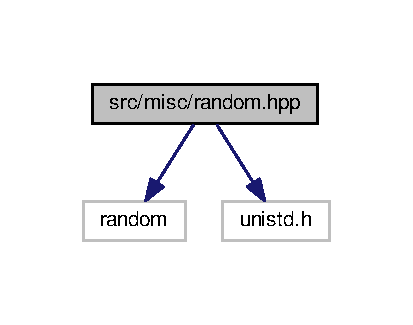
\includegraphics[width=204pt]{random_8hpp__incl}
\end{center}
\end{figure}
This graph shows which files directly or indirectly include this file\-:
\nopagebreak
\begin{figure}[H]
\begin{center}
\leavevmode
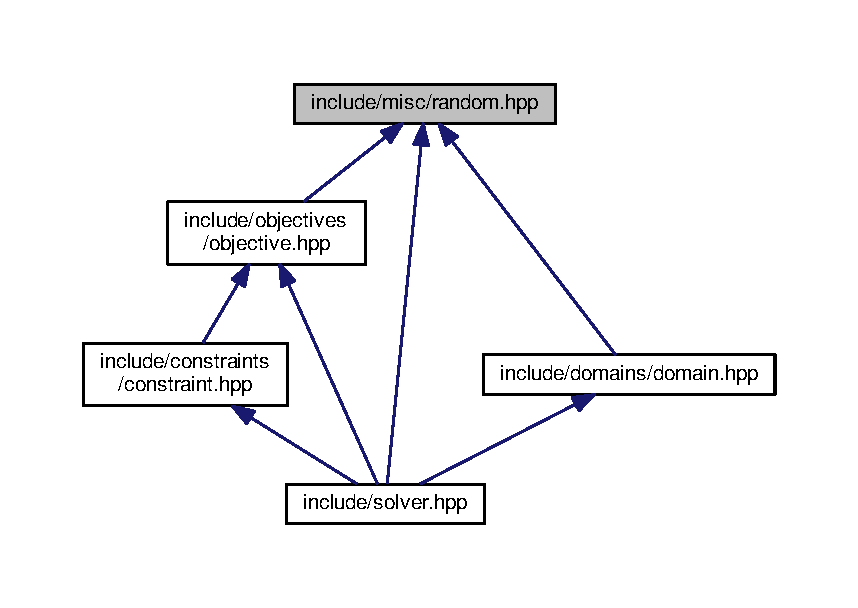
\includegraphics[width=350pt]{random_8hpp__dep__incl}
\end{center}
\end{figure}
\subsection*{Classes}
\begin{DoxyCompactItemize}
\item 
class \hyperlink{classghost_1_1Random}{ghost\-::\-Random}
\begin{DoxyCompactList}\small\item\em \hyperlink{classghost_1_1Random}{Random} is the class coding pseudo-\/random generators used in G\-H\-O\-S\-T. \end{DoxyCompactList}\end{DoxyCompactItemize}
\subsection*{Namespaces}
\begin{DoxyCompactItemize}
\item 
\hyperlink{namespaceghost}{ghost}
\end{DoxyCompactItemize}

\hypertarget{objective_8hpp}{\section{include/objectives/objective.hpp File Reference}
\label{objective_8hpp}\index{include/objectives/objective.\-hpp@{include/objectives/objective.\-hpp}}
}
{\ttfamily \#include $<$algorithm$>$}\\*
{\ttfamily \#include $<$limits$>$}\\*
{\ttfamily \#include $<$vector$>$}\\*
{\ttfamily \#include \char`\"{}../misc/random.\-hpp\char`\"{}}\\*
Include dependency graph for objective.\-hpp\-:
\nopagebreak
\begin{figure}[H]
\begin{center}
\leavevmode
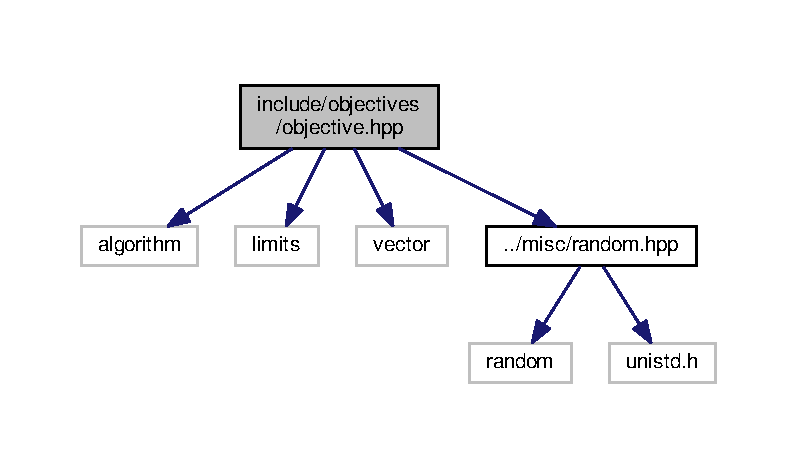
\includegraphics[width=350pt]{objective_8hpp__incl}
\end{center}
\end{figure}
This graph shows which files directly or indirectly include this file\-:
\nopagebreak
\begin{figure}[H]
\begin{center}
\leavevmode
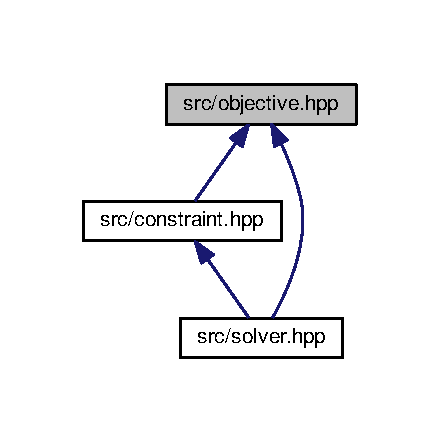
\includegraphics[width=350pt]{objective_8hpp__dep__incl}
\end{center}
\end{figure}
\subsection*{Classes}
\begin{DoxyCompactItemize}
\item 
class \hyperlink{classghost_1_1Objective}{ghost\-::\-Objective$<$ Type\-Variable, Type\-Domain $>$}
\begin{DoxyCompactList}\small\item\em \hyperlink{classghost_1_1Objective}{Objective} is the class encoding objective functions of your C\-S\-P/\-C\-O\-P. \end{DoxyCompactList}\item 
class \hyperlink{classghost_1_1NullObjective}{ghost\-::\-Null\-Objective$<$ Type\-Variable, Type\-Domain $>$}
\begin{DoxyCompactList}\small\item\em \hyperlink{classghost_1_1NullObjective}{Null\-Objective} is used when no objective functions have been given to the solver (ie, for pure satisfaction runs). \end{DoxyCompactList}\end{DoxyCompactItemize}
\subsection*{Namespaces}
\begin{DoxyCompactItemize}
\item 
\hyperlink{namespaceghost}{ghost}
\end{DoxyCompactItemize}

\hypertarget{solver_8hpp}{\section{include/solver.hpp File Reference}
\label{solver_8hpp}\index{include/solver.\-hpp@{include/solver.\-hpp}}
}
{\ttfamily \#include $<$vector$>$}\\*
{\ttfamily \#include $<$set$>$}\\*
{\ttfamily \#include $<$memory$>$}\\*
{\ttfamily \#include $<$cmath$>$}\\*
{\ttfamily \#include $<$chrono$>$}\\*
{\ttfamily \#include $<$ctime$>$}\\*
{\ttfamily \#include $<$limits$>$}\\*
{\ttfamily \#include $<$algorithm$>$}\\*
{\ttfamily \#include $<$functional$>$}\\*
{\ttfamily \#include $<$cassert$>$}\\*
{\ttfamily \#include $<$typeinfo$>$}\\*
{\ttfamily \#include \char`\"{}variable.\-hpp\char`\"{}}\\*
{\ttfamily \#include \char`\"{}constraint.\-hpp\char`\"{}}\\*
{\ttfamily \#include \char`\"{}domain.\-hpp\char`\"{}}\\*
{\ttfamily \#include \char`\"{}misc/random.\-hpp\char`\"{}}\\*
{\ttfamily \#include \char`\"{}objective.\-hpp\char`\"{}}\\*
Include dependency graph for solver.\-hpp\-:\nopagebreak
\begin{figure}[H]
\begin{center}
\leavevmode
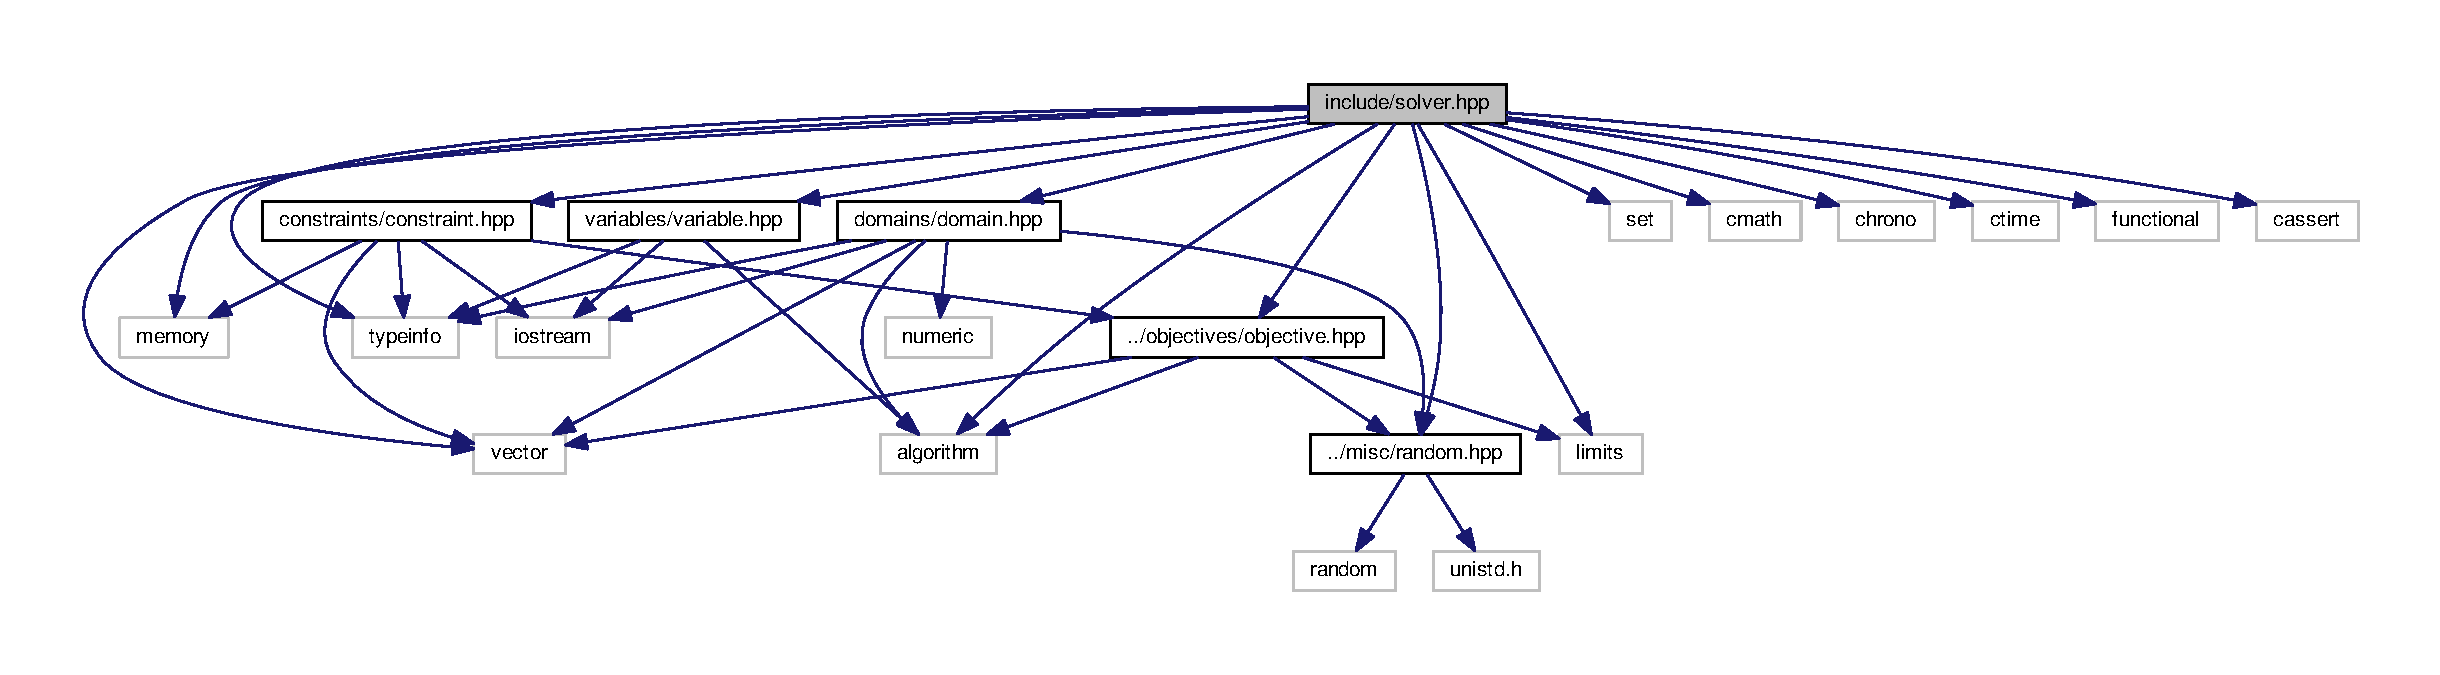
\includegraphics[width=350pt]{solver_8hpp__incl}
\end{center}
\end{figure}
\subsection*{Classes}
\begin{DoxyCompactItemize}
\item 
class \hyperlink{classghost_1_1Solver}{ghost\-::\-Solver$<$ Type\-Variable, Type\-Domain, Type\-Constraint $>$}
\begin{DoxyCompactList}\small\item\em \hyperlink{classghost_1_1Solver}{Solver} is the class coding the solver itself. \end{DoxyCompactList}\end{DoxyCompactItemize}
\subsection*{Namespaces}
\begin{DoxyCompactItemize}
\item 
\hyperlink{namespaceghost}{ghost}
\end{DoxyCompactItemize}

\hypertarget{variable_8hpp}{}\section{include/variable.hpp File Reference}
\label{variable_8hpp}\index{include/variable.\+hpp@{include/variable.\+hpp}}
{\ttfamily \#include $<$iostream$>$}\\*
{\ttfamily \#include $<$vector$>$}\\*
{\ttfamily \#include \char`\"{}domain.\+hpp\char`\"{}}\\*
Include dependency graph for variable.\+hpp\+:\nopagebreak
\begin{figure}[H]
\begin{center}
\leavevmode
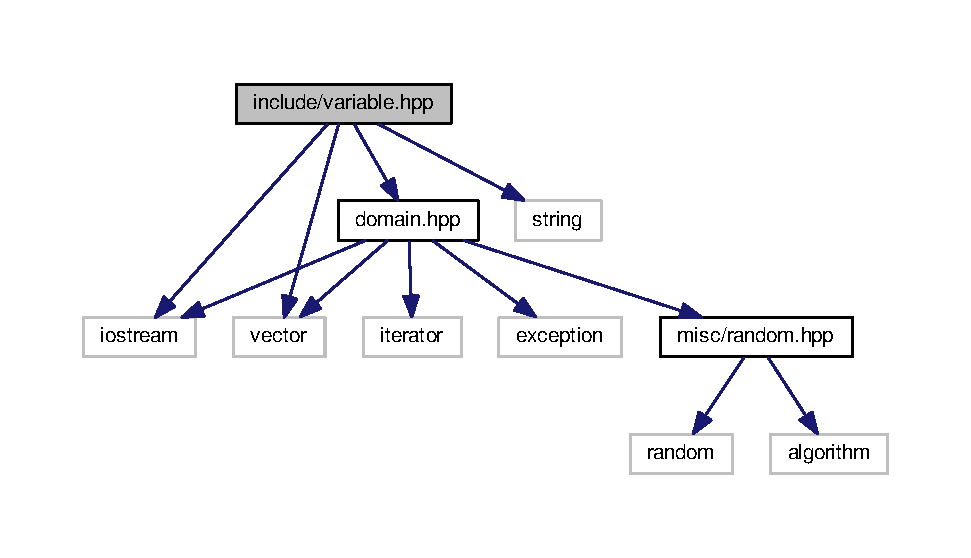
\includegraphics[width=350pt]{variable_8hpp__incl}
\end{center}
\end{figure}
This graph shows which files directly or indirectly include this file\+:\nopagebreak
\begin{figure}[H]
\begin{center}
\leavevmode
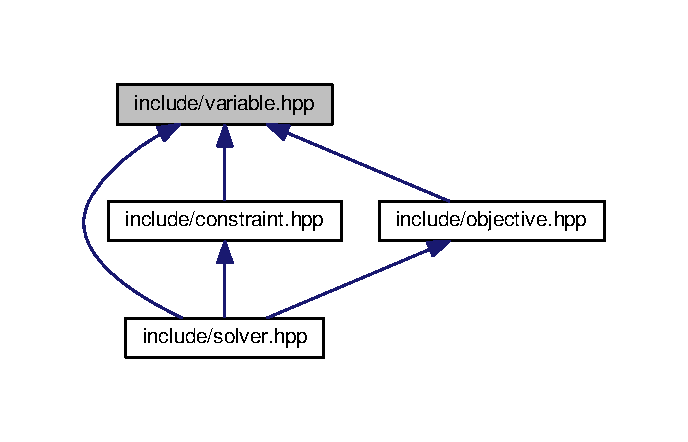
\includegraphics[width=330pt]{variable_8hpp__dep__incl}
\end{center}
\end{figure}
\subsection*{Classes}
\begin{DoxyCompactItemize}
\item 
class \hyperlink{classghost_1_1Variable}{ghost\+::\+Variable}
\begin{DoxyCompactList}\small\item\em This class encodes variables of your C\+S\+P/\+C\+OP. You cannot inherits your own class from \hyperlink{classghost_1_1Variable}{Variable}. \end{DoxyCompactList}\end{DoxyCompactItemize}
\subsection*{Namespaces}
\begin{DoxyCompactItemize}
\item 
 \hyperlink{namespaceghost}{ghost}
\end{DoxyCompactItemize}

%--- End generated contents ---

% Index
\newpage
\phantomsection
\addcontentsline{toc}{chapter}{Index}
\printindex

\end{document}
